\chapter{Galería de gráficas}\label{ap:galeria}

Este apéndice reúne las gráficas completas que en el cuerpo del documento aparecen resumidas o recortadas a las seis
canciones del álbum. Se ordenan por dimensión, en el mismo orden que el capítulo~\ref{cap:resultados}: armonía, melodía,
síntesis y, al final, los radares de estilo de la primera versión de la comparación
(sección~\ref{sec:primeras-comparaciones}). Todas incluyen las 36 canciones medidas: las seis de la banda, los tres
controles de Primus y los repertorios de King Gizzard, Zappa, King Crimson y Gentle Giant.

\section{Armonía}

La matriz y el mapa de las figuras~\ref{fig:g-matriz} y~\ref{fig:g-mapa} amplían las figuras~\ref{fig:matriz} y~\ref{fig:mapa} a las 36 canciones. Las figuras~\ref{fig:g-distancias} a~\ref{fig:g-veredictos2} son de la versión con reglas (sección~\ref{sec:primeras-comparaciones}).

\begin{figure}[!htbp]
  \centering
  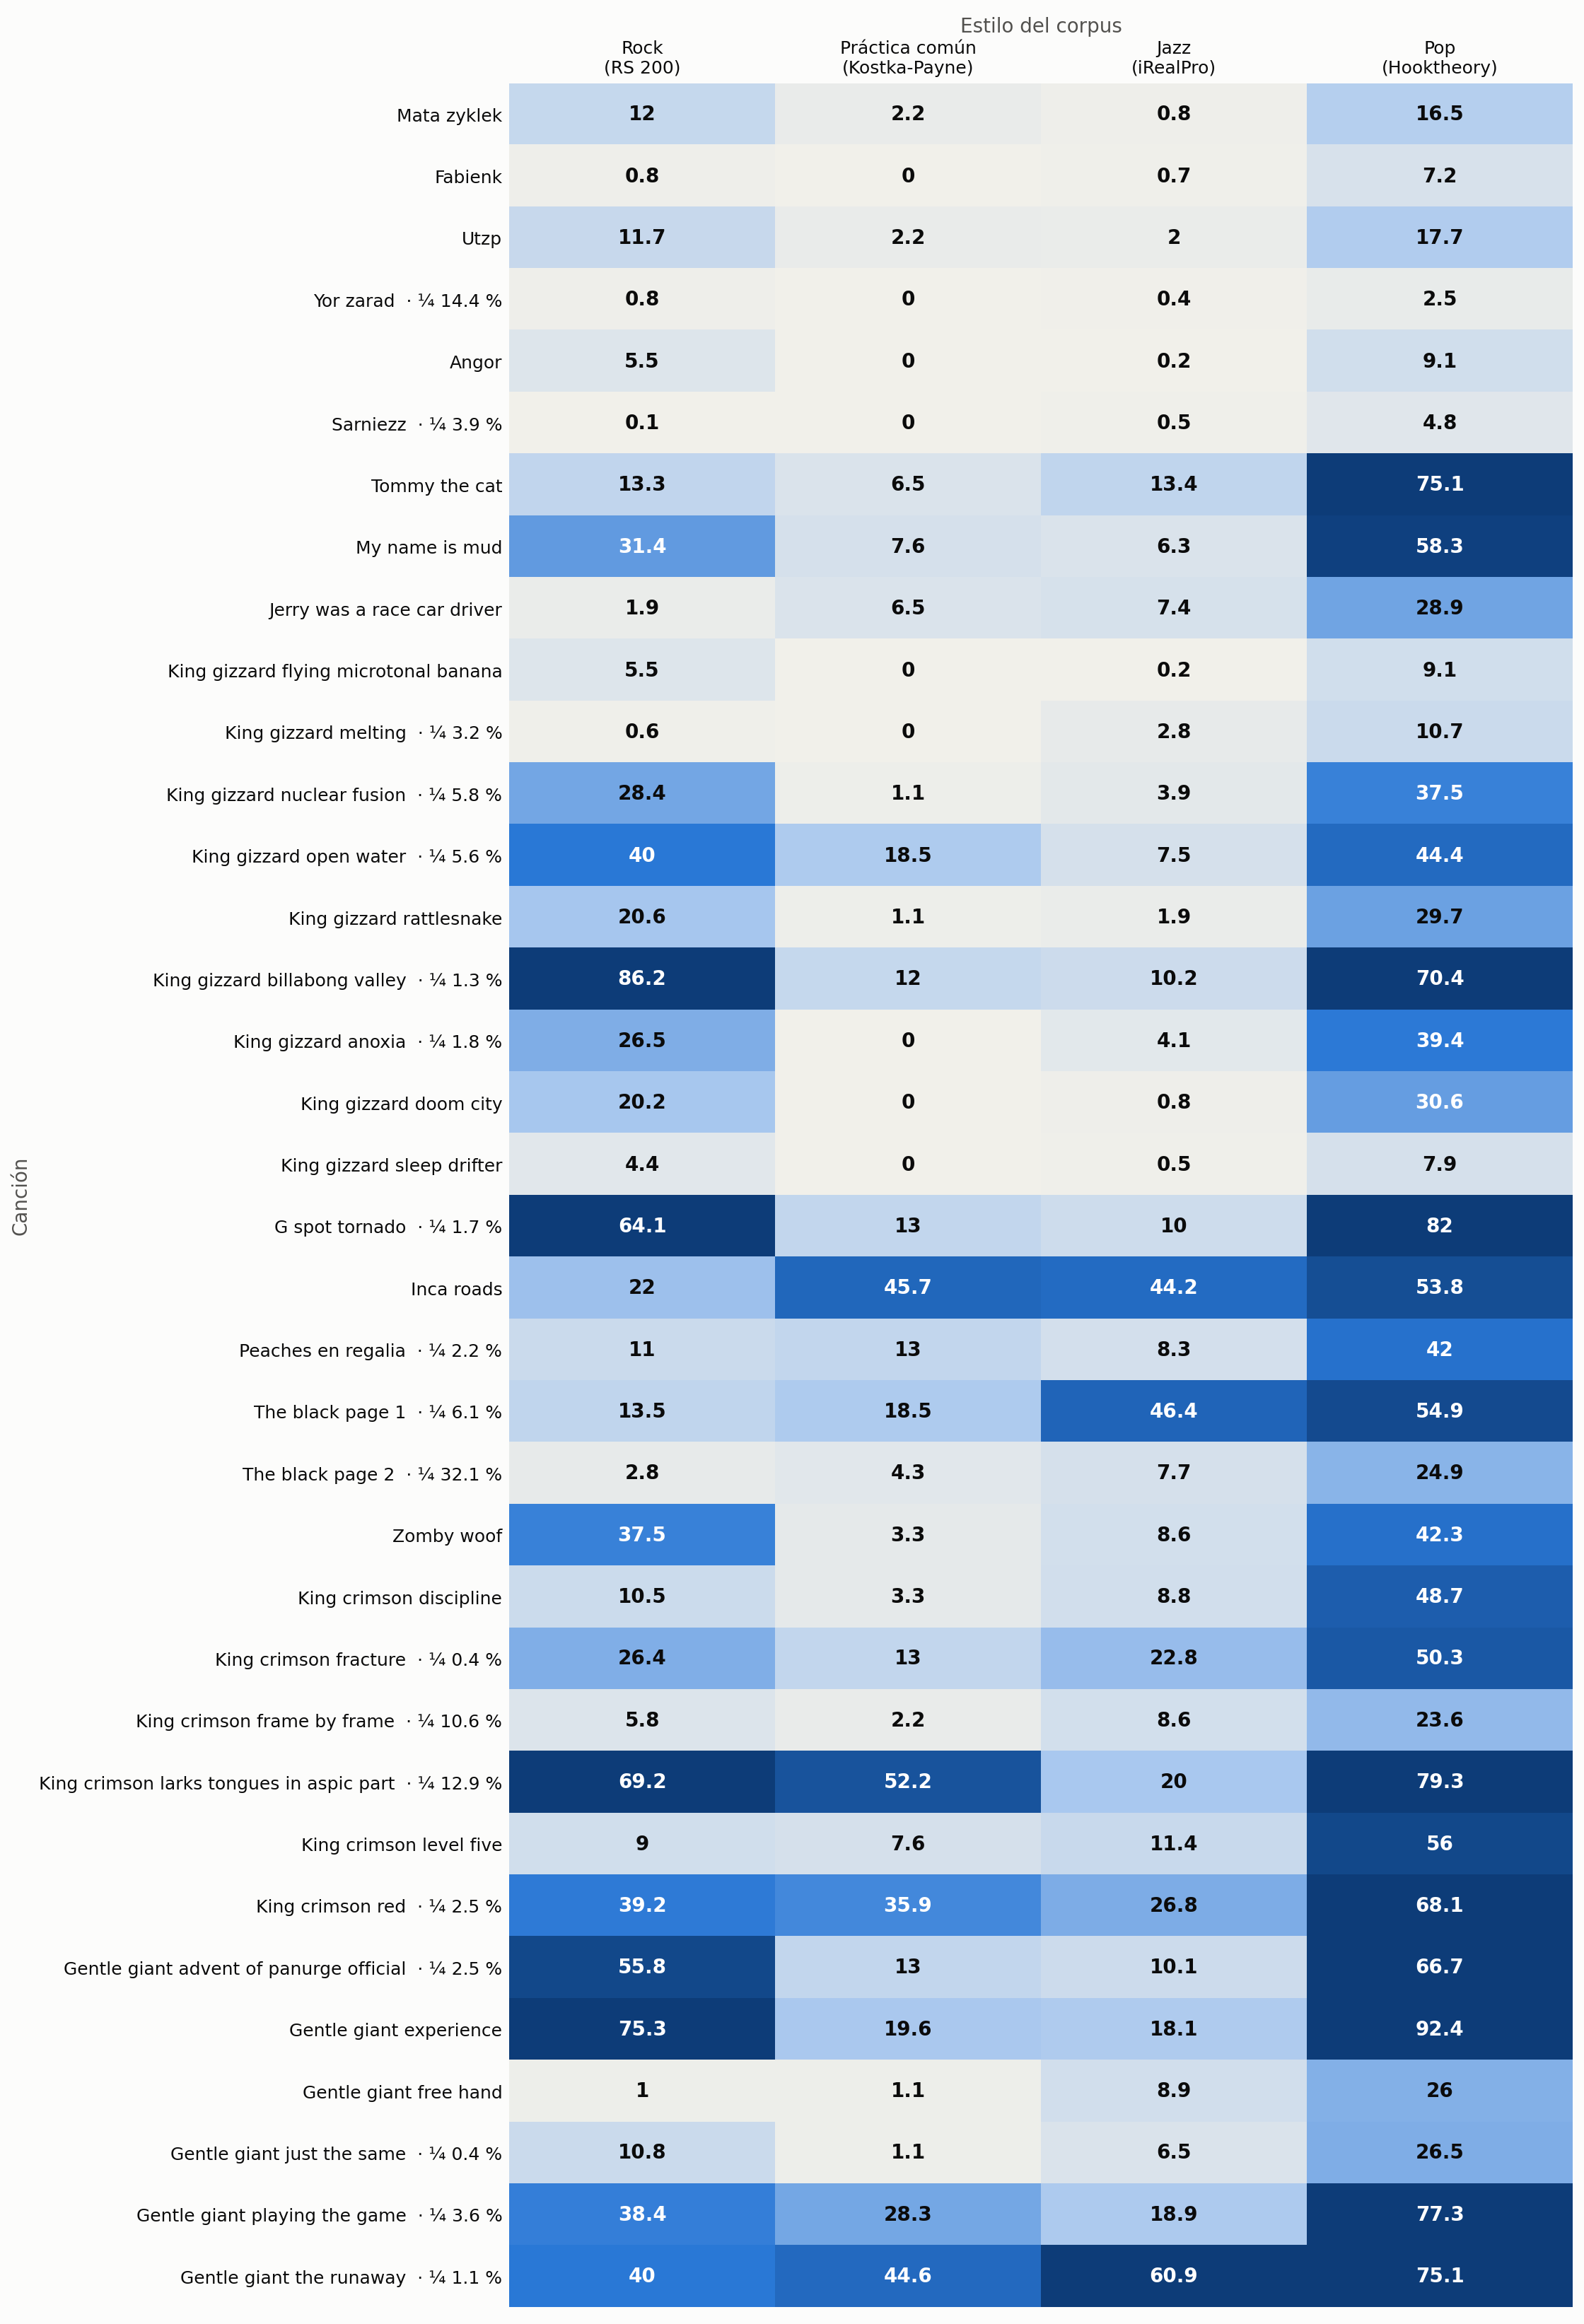
\includegraphics[width=\textwidth,height=0.78\textheight,keepaspectratio]{g_verosimilitud_matriz.png}
  \caption{Matriz de verosimilitud armónica de las 36 canciones frente a rock (RS~200, de Clercq y Temperley), práctica común (Kostka-Payne), jazz (iRealPro) y pop (9 álbumes de Hooktheory). Percentil: porcentaje de piezas del estilo tan o más alejadas que la canción (50 = típica). «¼\,\%»: tiempo con fundamental en cuarto de tono, llevada al grado de abajo.}\label{fig:g-matriz}
\end{figure}

\begin{figure}[!htbp]
  \centering
  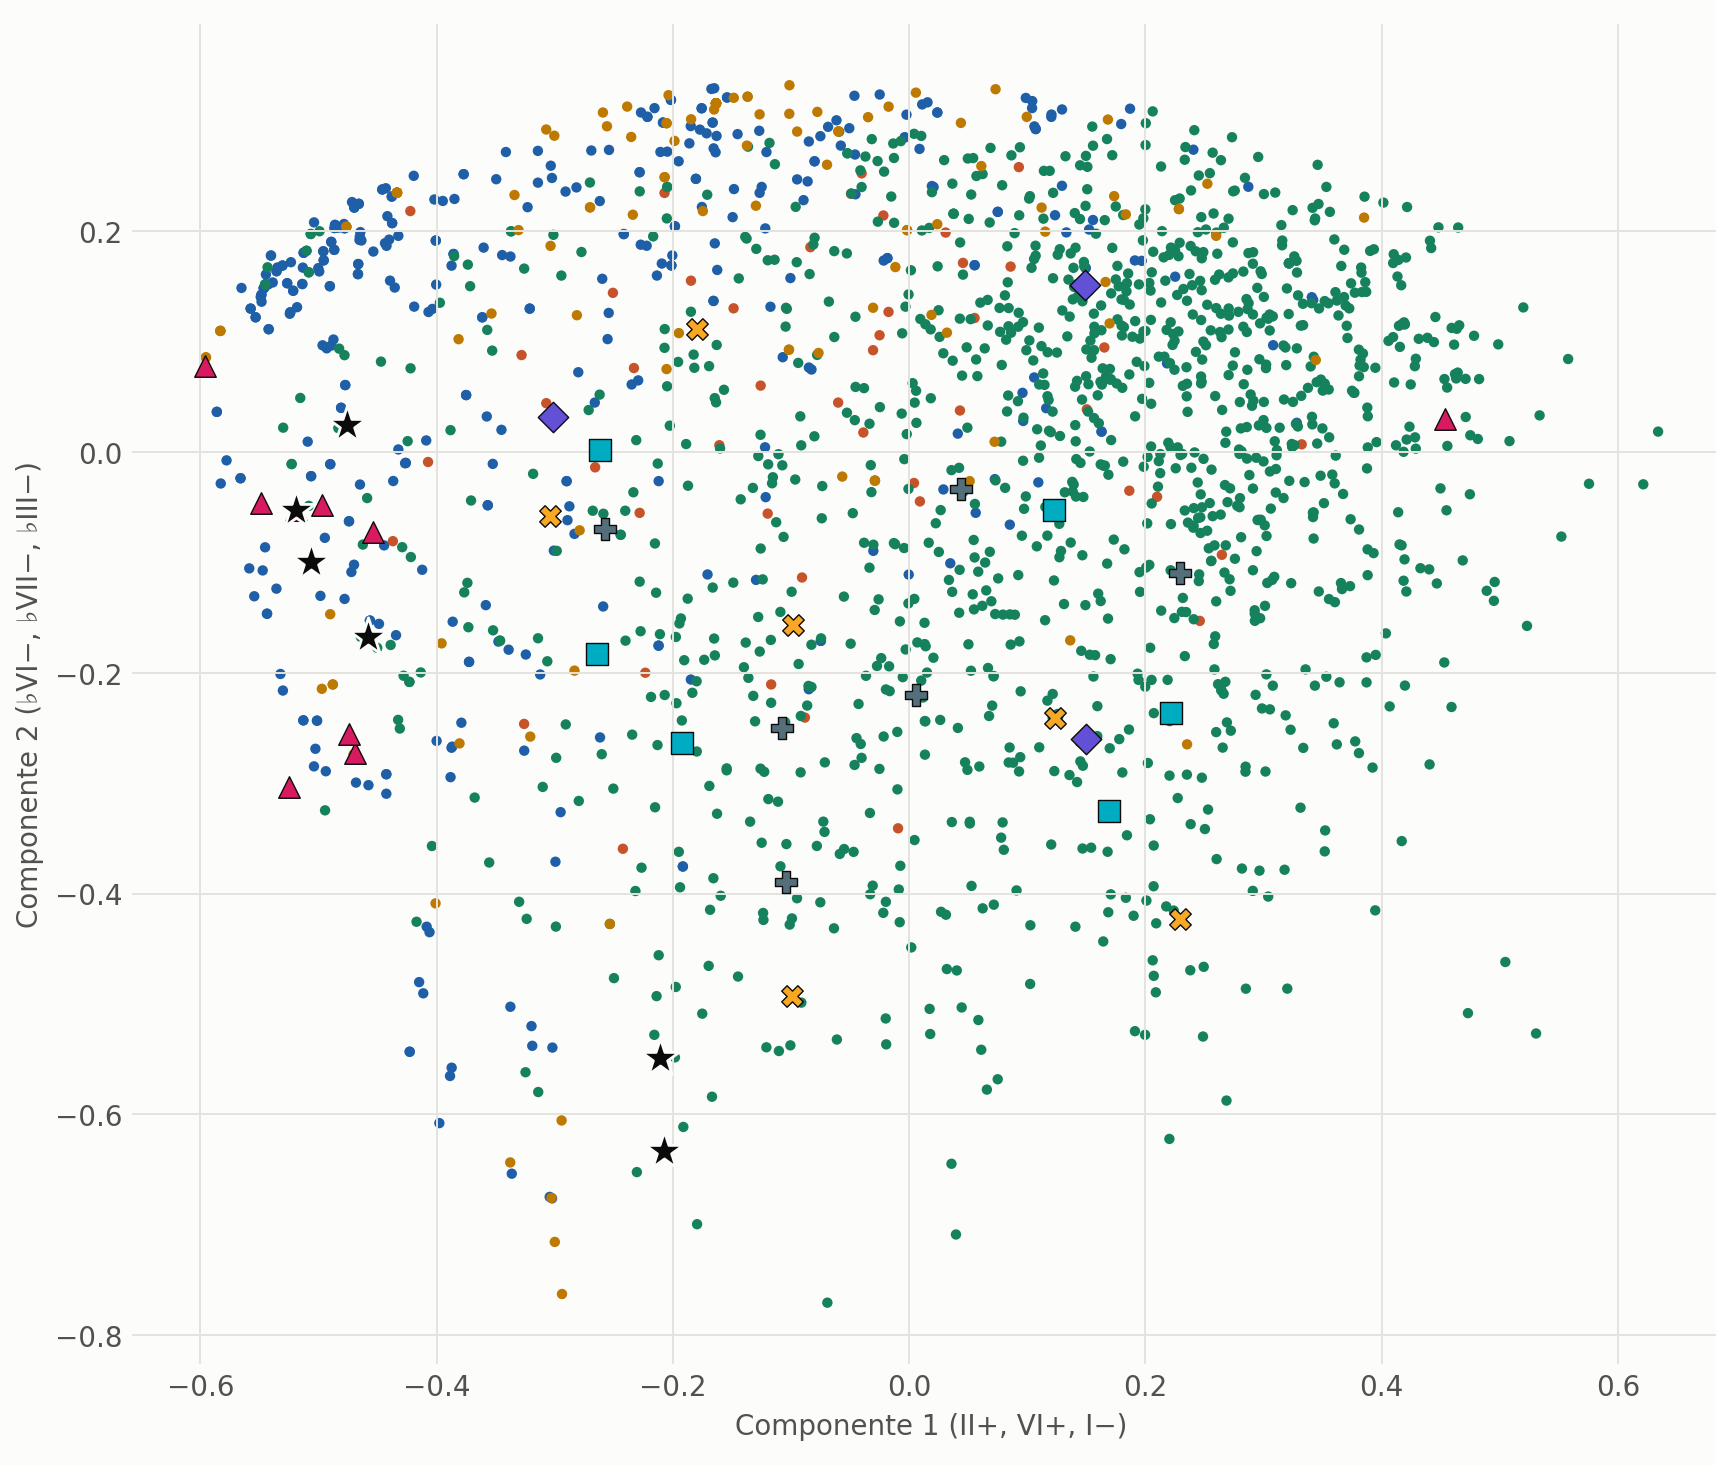
\includegraphics[width=\textwidth]{g_verosimilitud_mapa.png}
  \caption{Mapa de fundamentales de las 36 canciones. Puntos del fondo: rock (azul, RS~200, 400 piezas), práctica común (rojo, Kostka-Payne, 46), jazz (verde, iRealPro, 1186) y pop (naranja, Hooktheory, 121). Símbolos: estrella negra, la banda; rombo violeta, Primus; triángulo rosa, King Gizzard; cuadrado turquesa, Zappa; cruz gris, King Crimson; aspa amarilla, Gentle Giant.}
  \label{fig:g-mapa}
\end{figure}

\begin{figure}[!htbp]
  \centering
  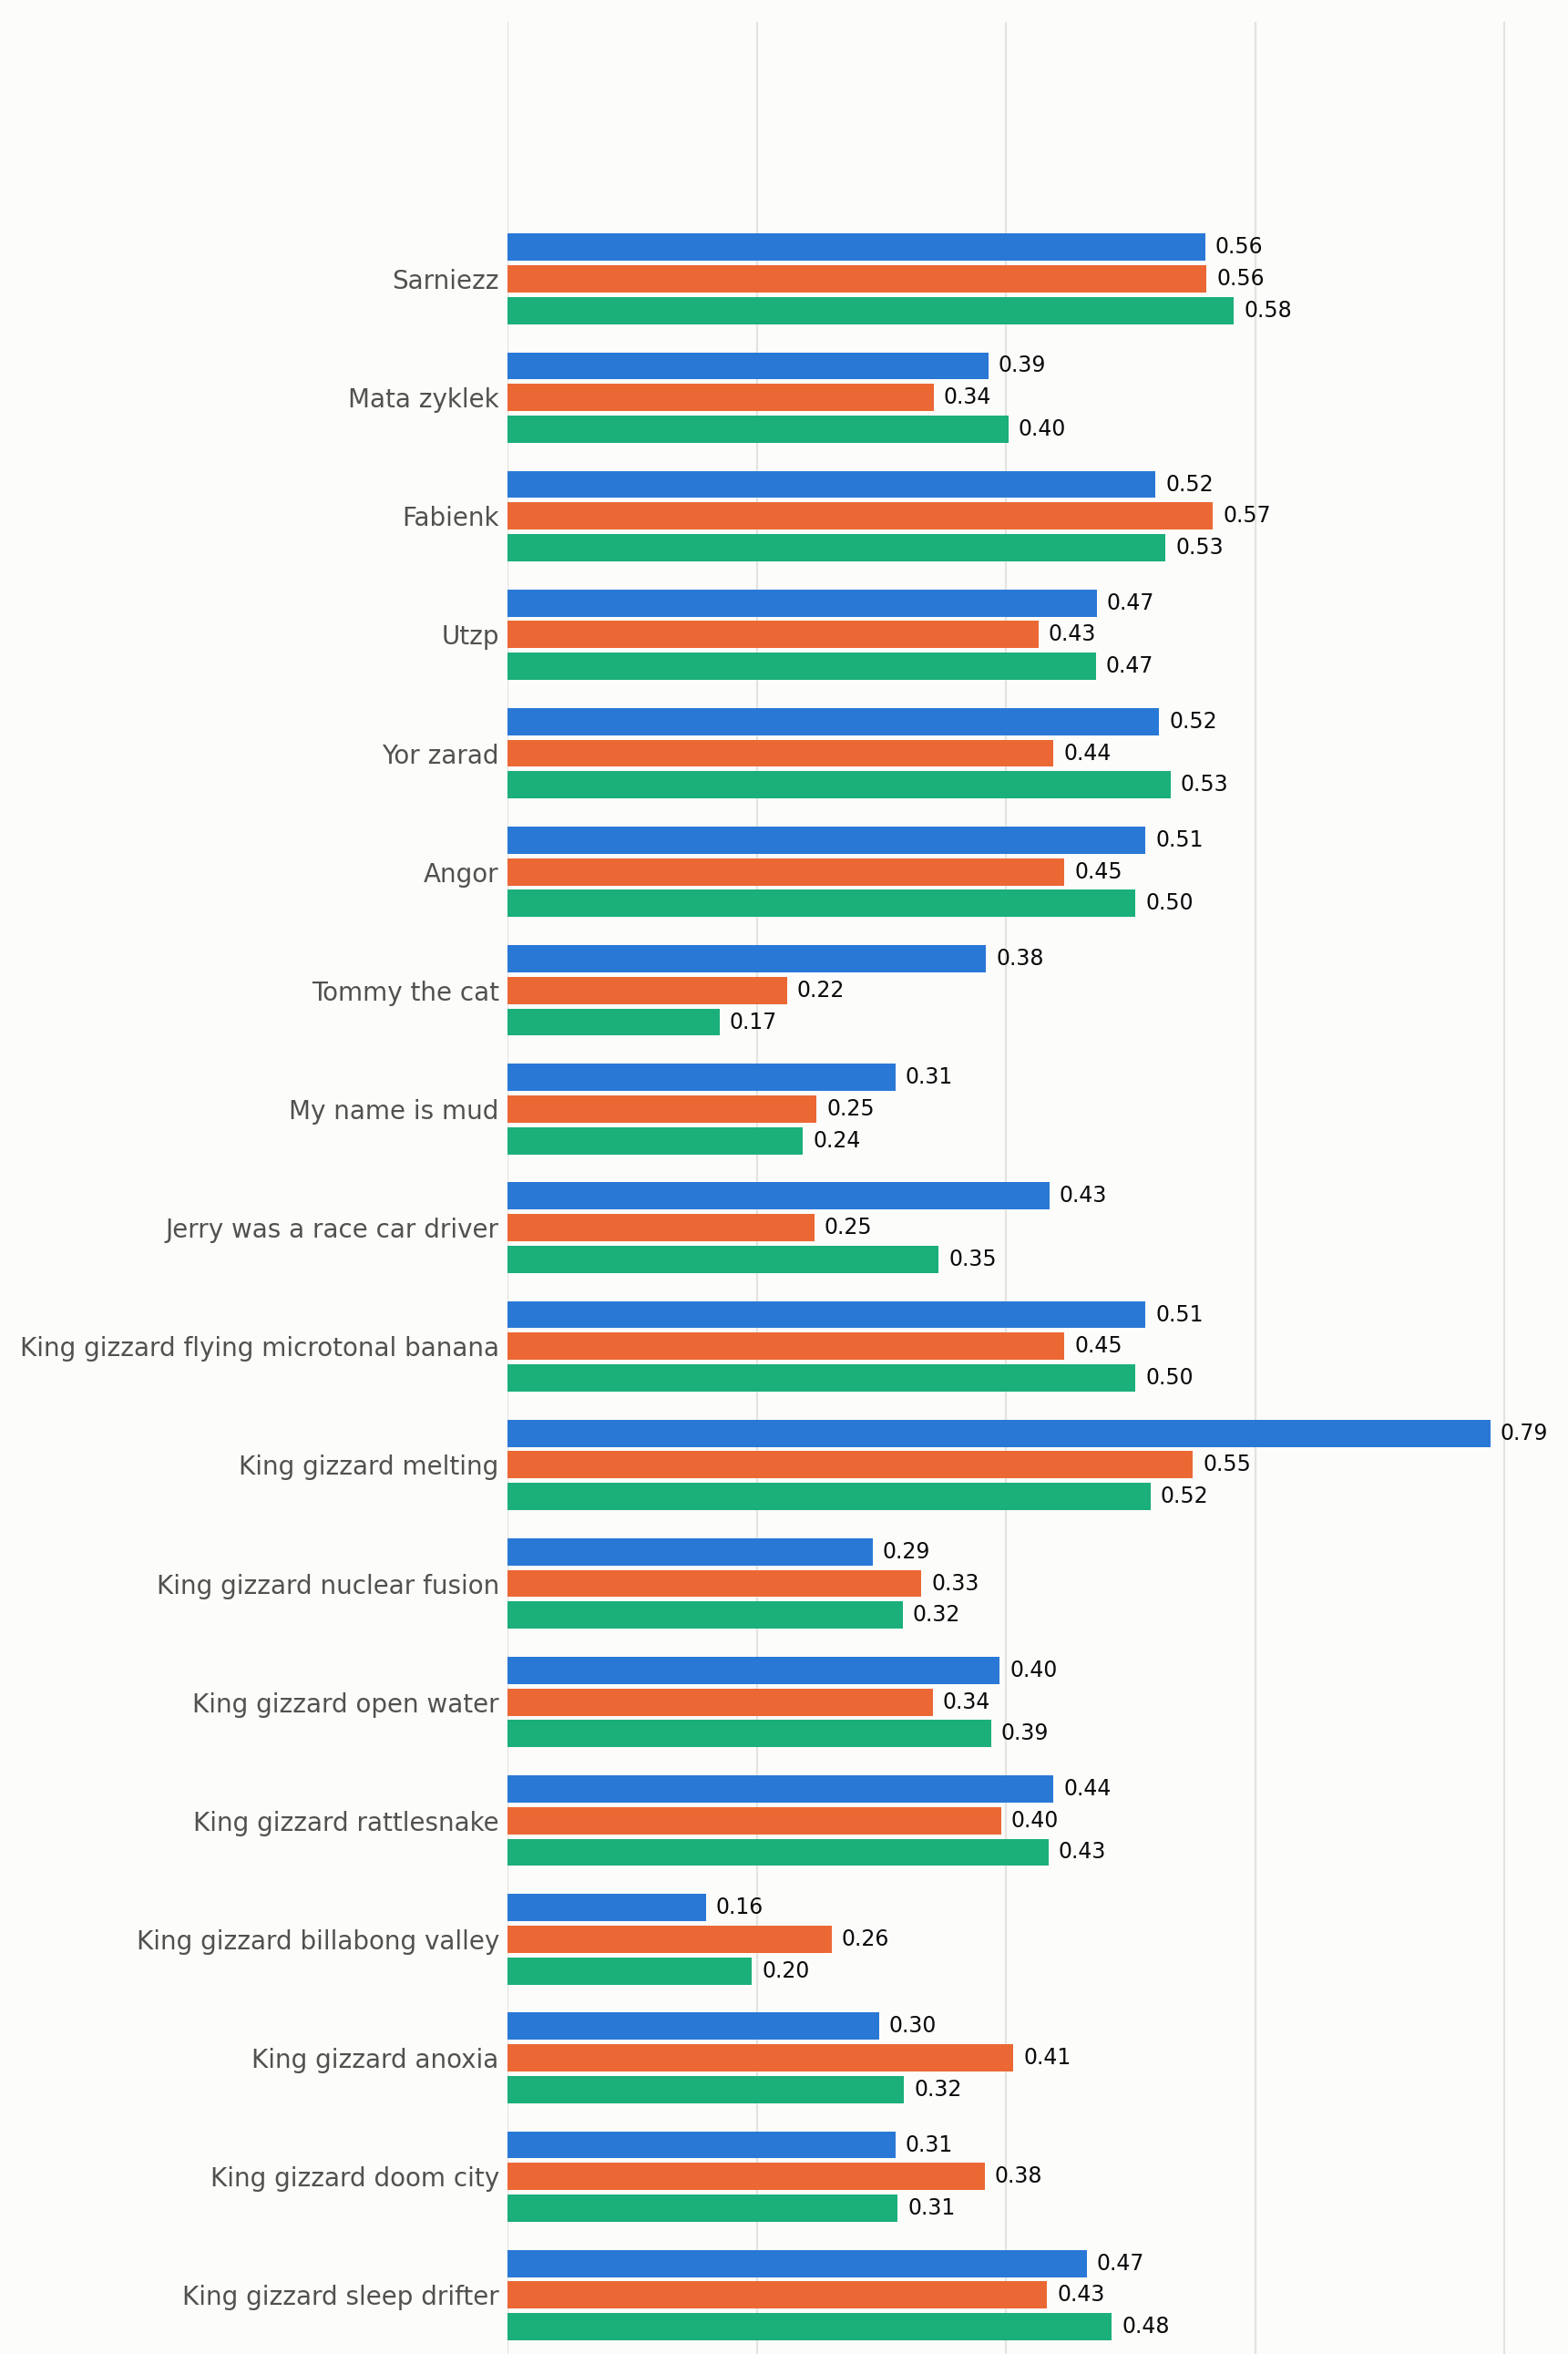
\includegraphics[width=0.495\textwidth]{g_distancias_estilos_a.png}\hfill
  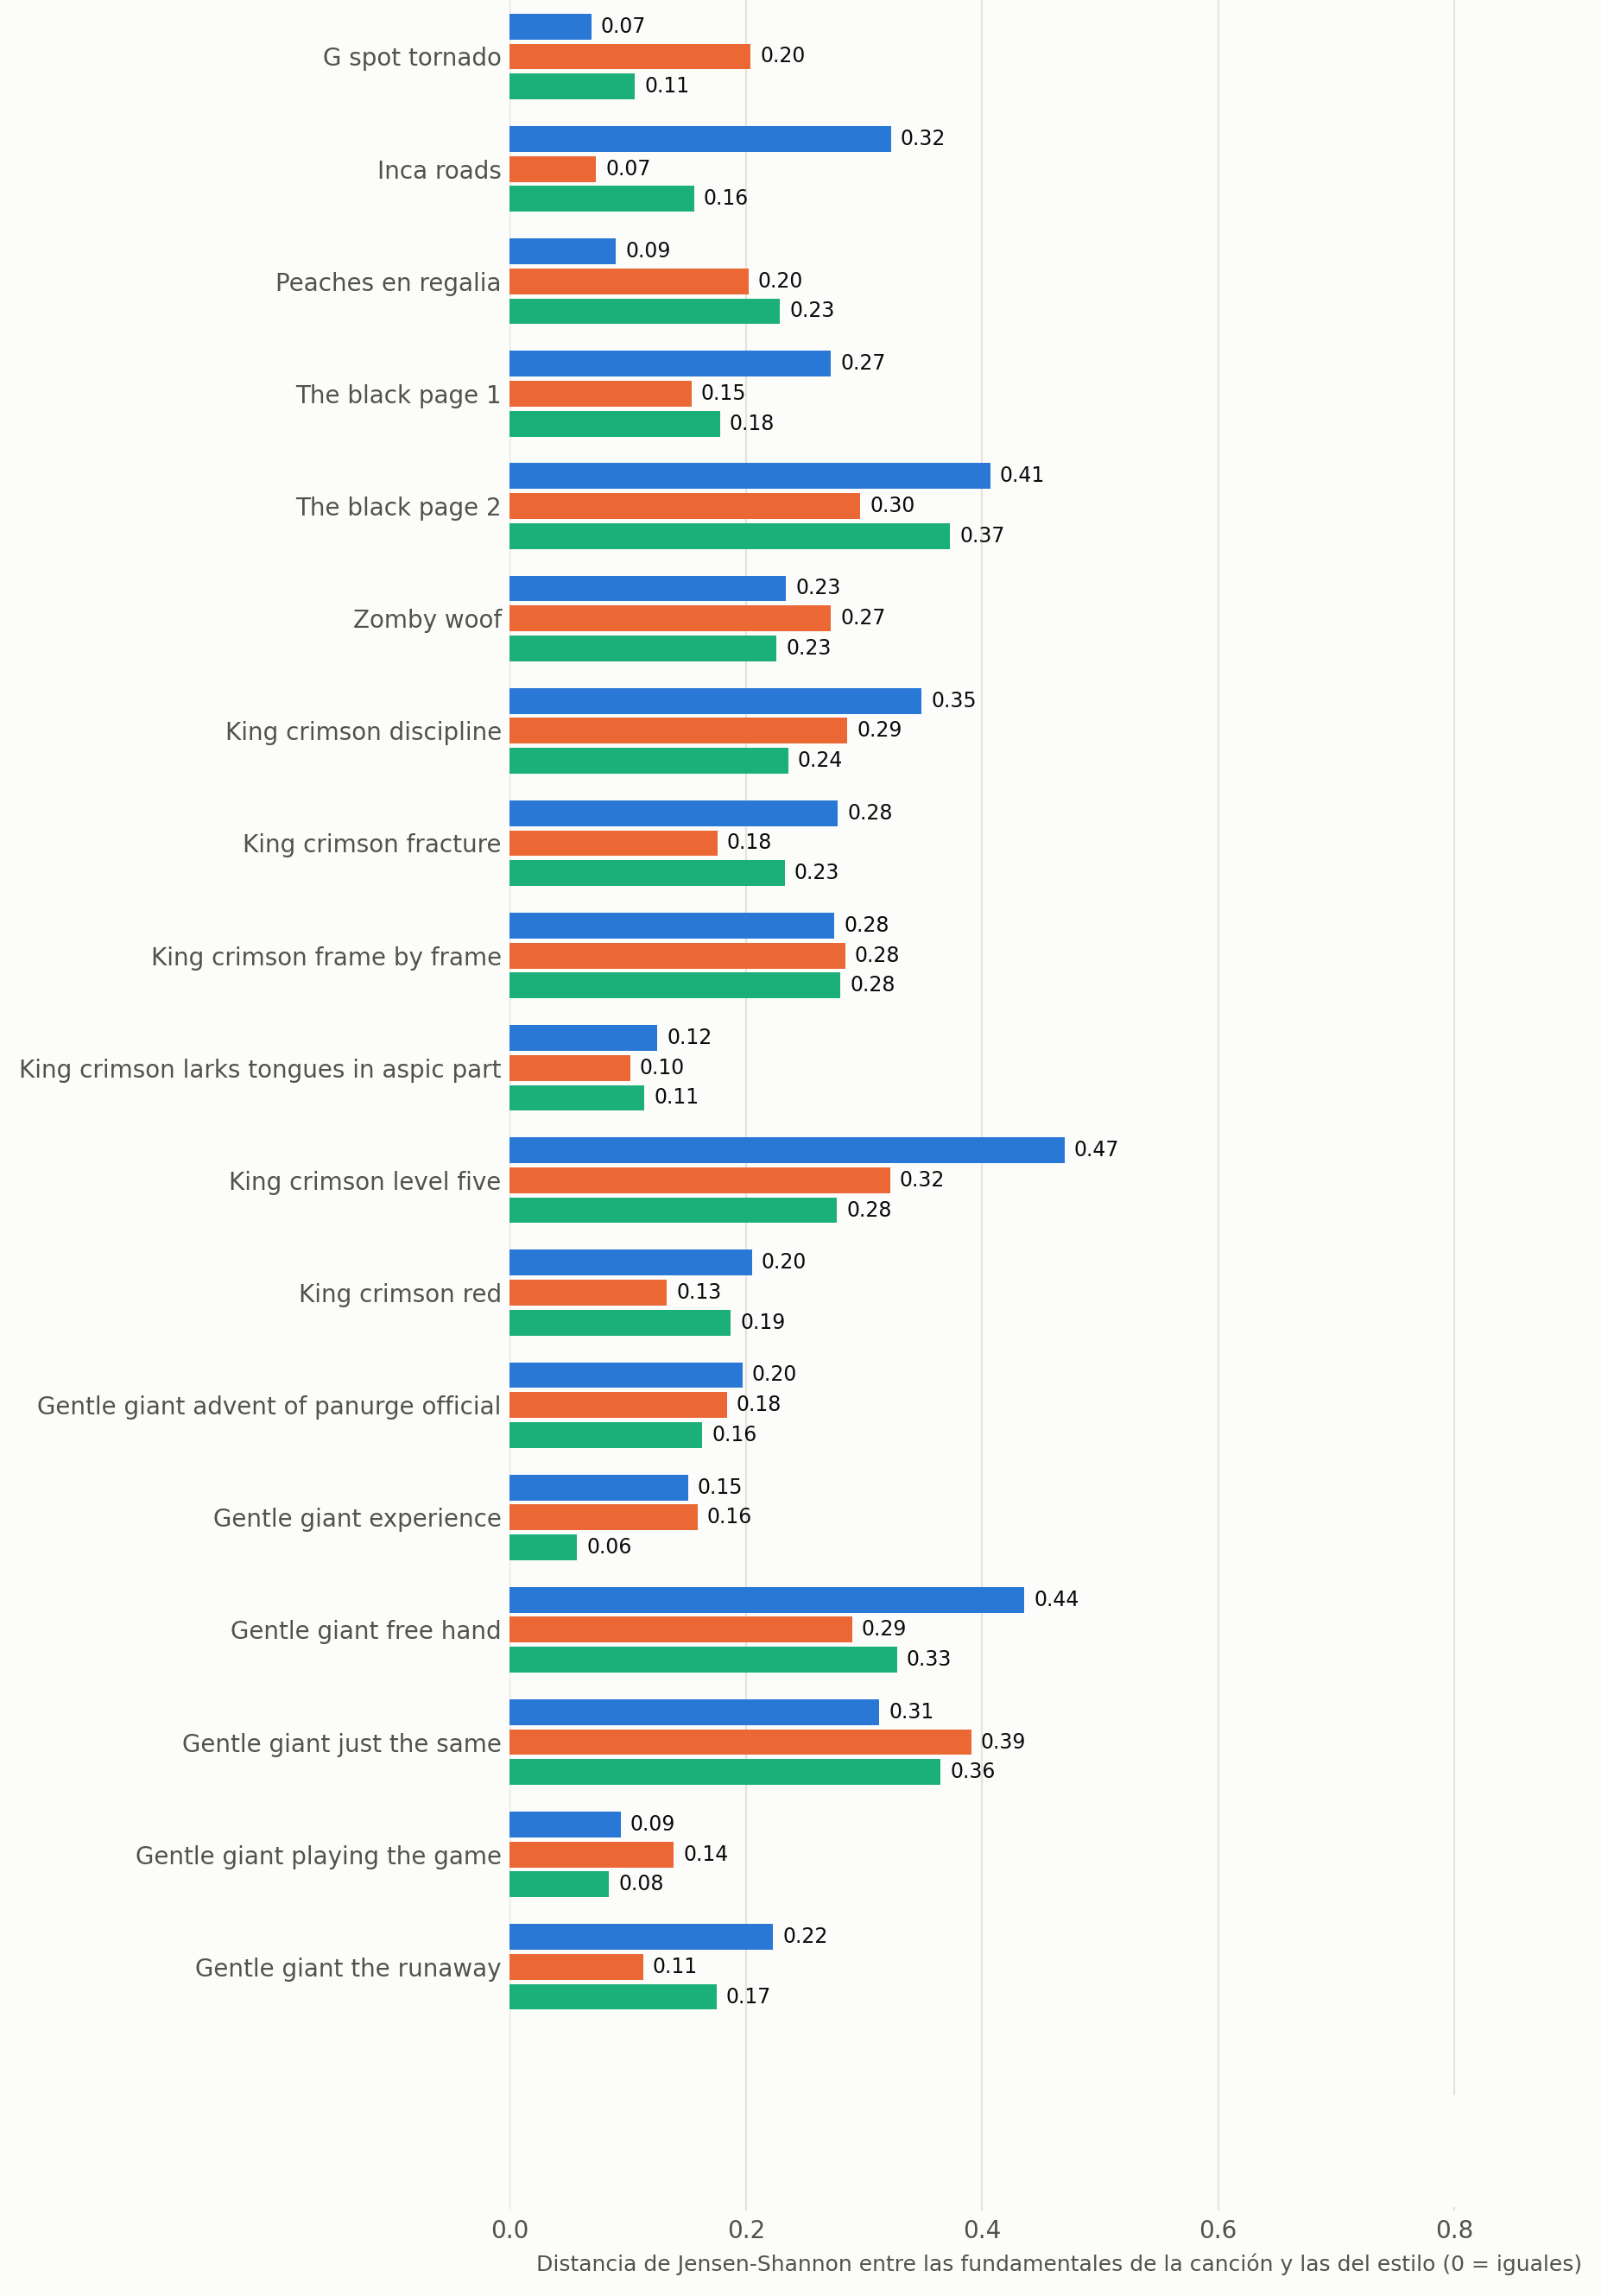
\includegraphics[width=0.495\textwidth]{g_distancias_estilos_b.png}
  \caption{Distancia de Jensen-Shannon de las fundamentales de cada canción a rock (azul, 100 canciones), práctica común (naranja) y pop (verde, 9 álbumes); 0 = iguales. Las canciones siguen en la columna derecha. Versión con reglas, descartada.}
  \label{fig:g-distancias}
\end{figure}

\begin{figure}[!htbp]
  \centering
  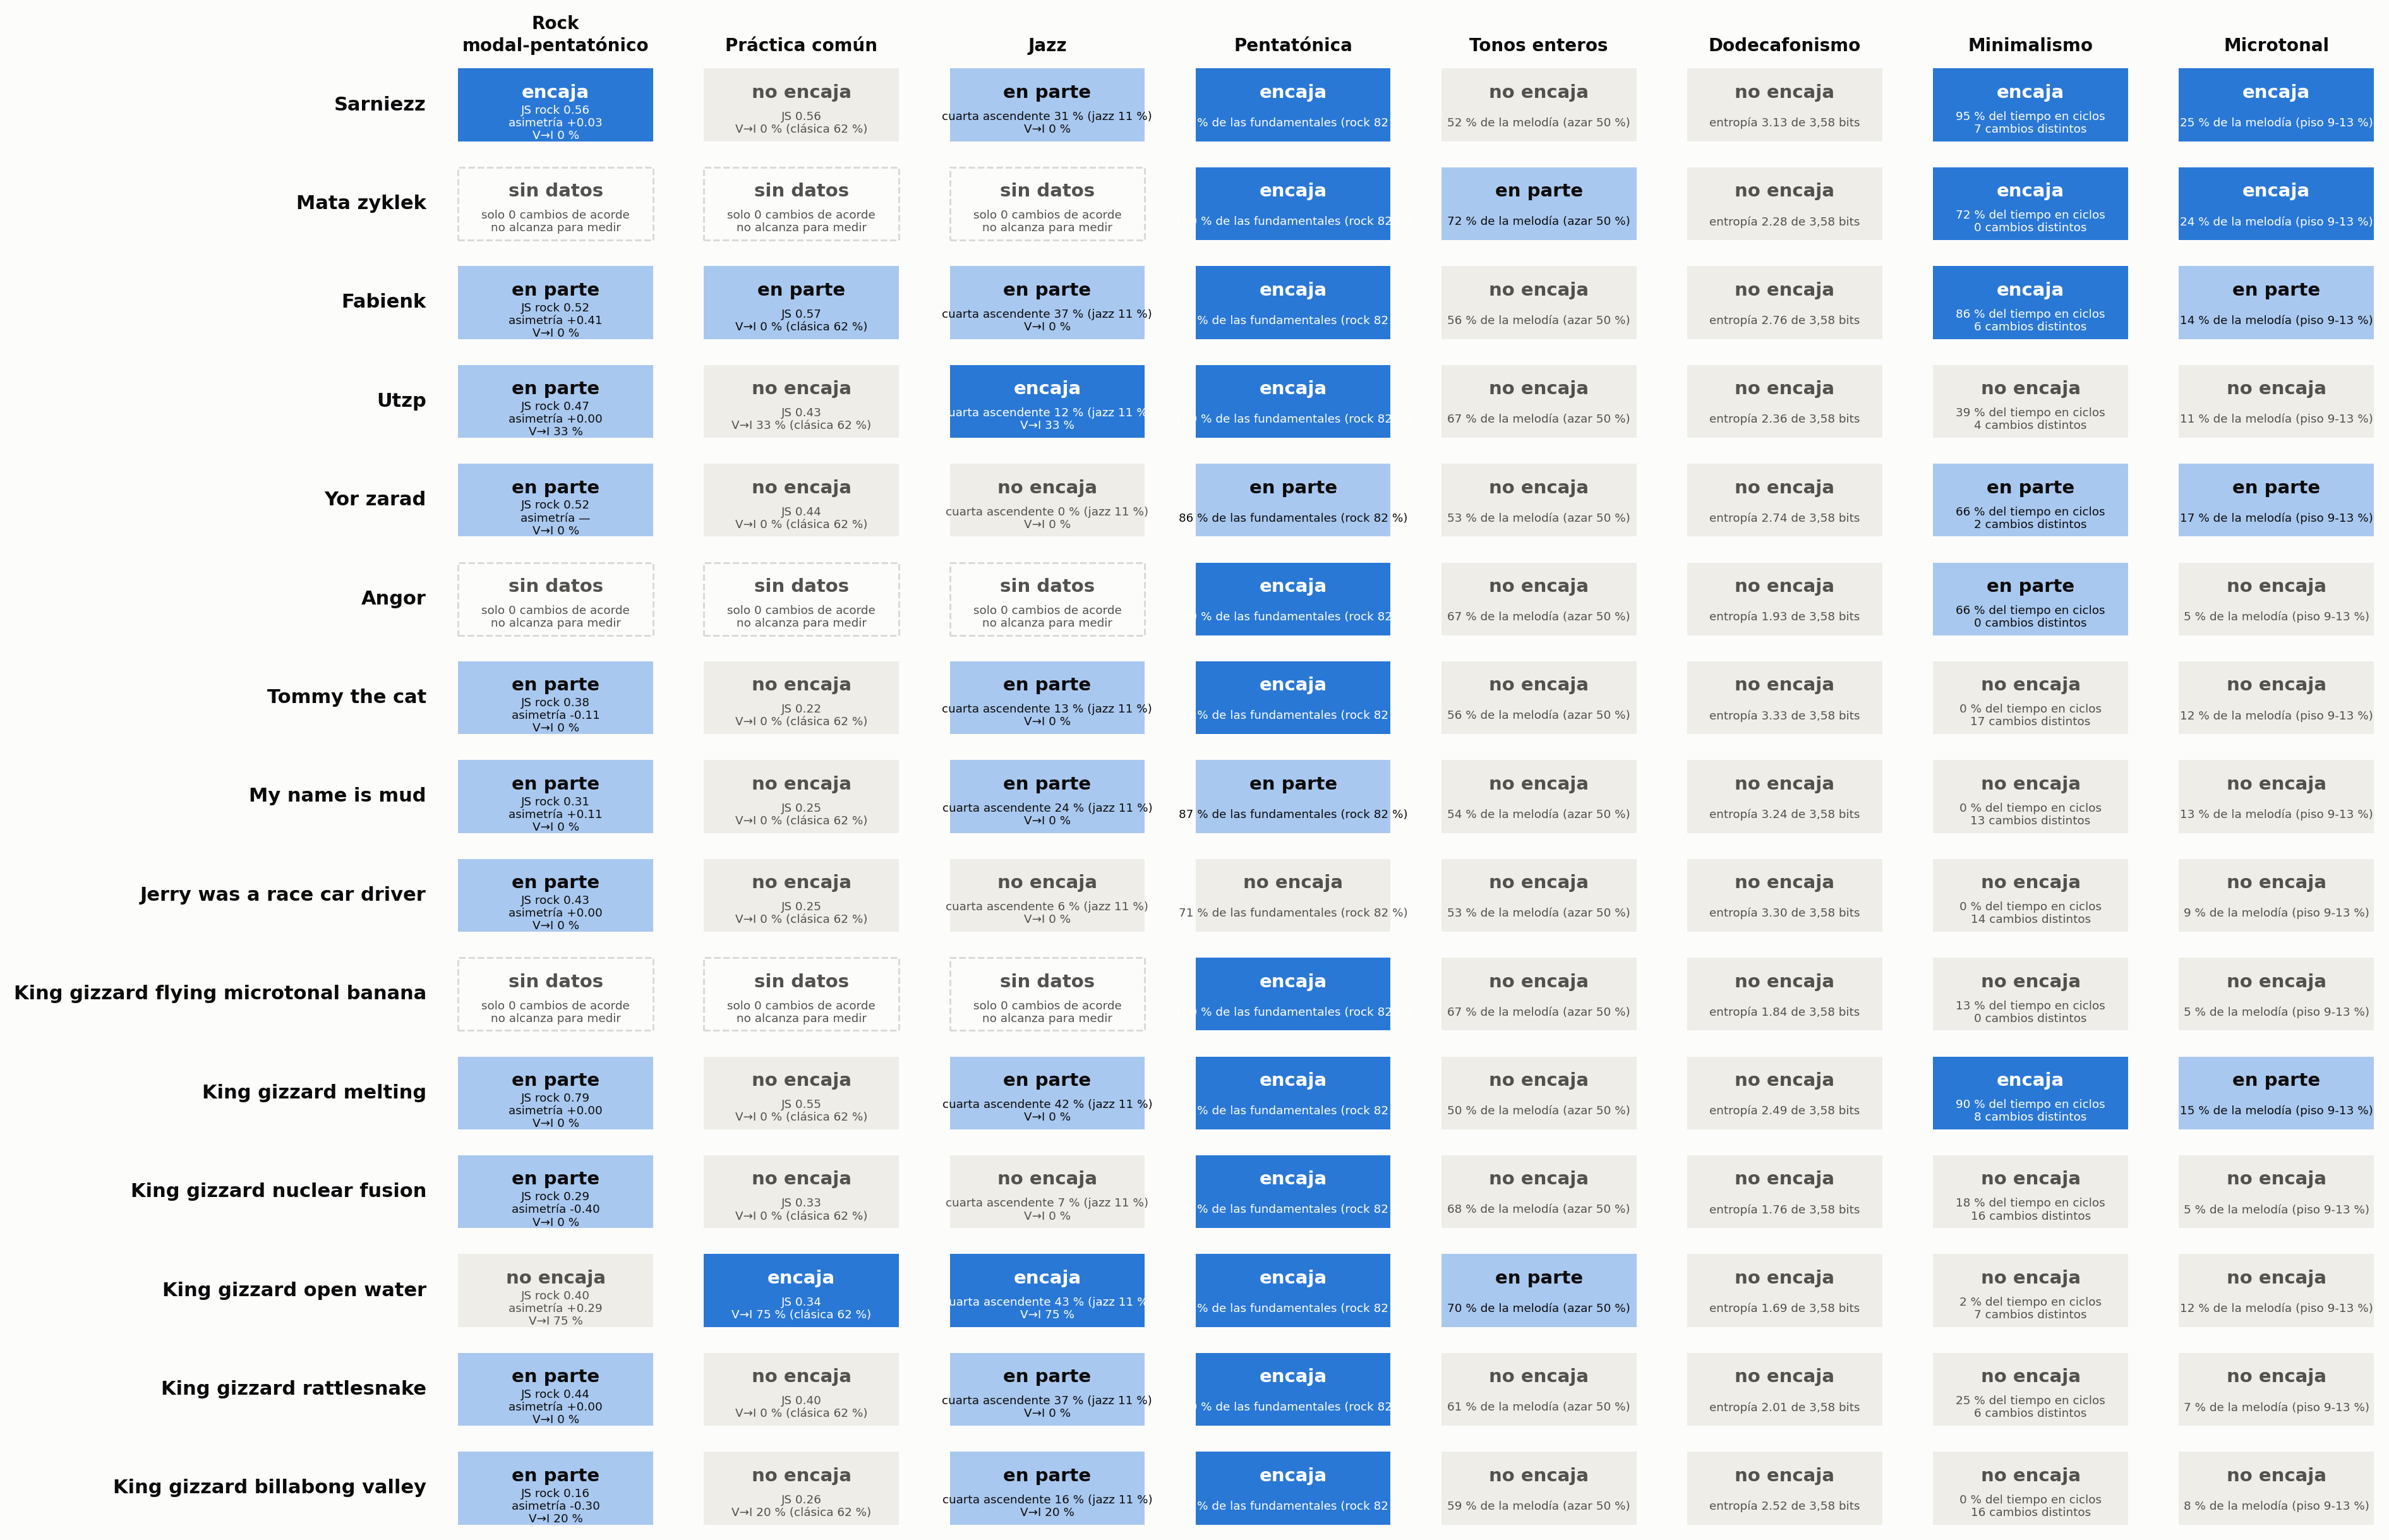
\includegraphics[width=\textwidth,height=0.78\textheight,keepaspectratio]{g_veredictos_estilos_1.png}
  \caption{Pruebas de estilo con reglas, canciones 1--15 (versión descartada). Azul oscuro: encaja; azul claro: encaja en parte; gris: no encaja; blanco: sin datos.}\label{fig:g-veredictos1}
\end{figure}

\begin{figure}[!htbp]
  \centering
  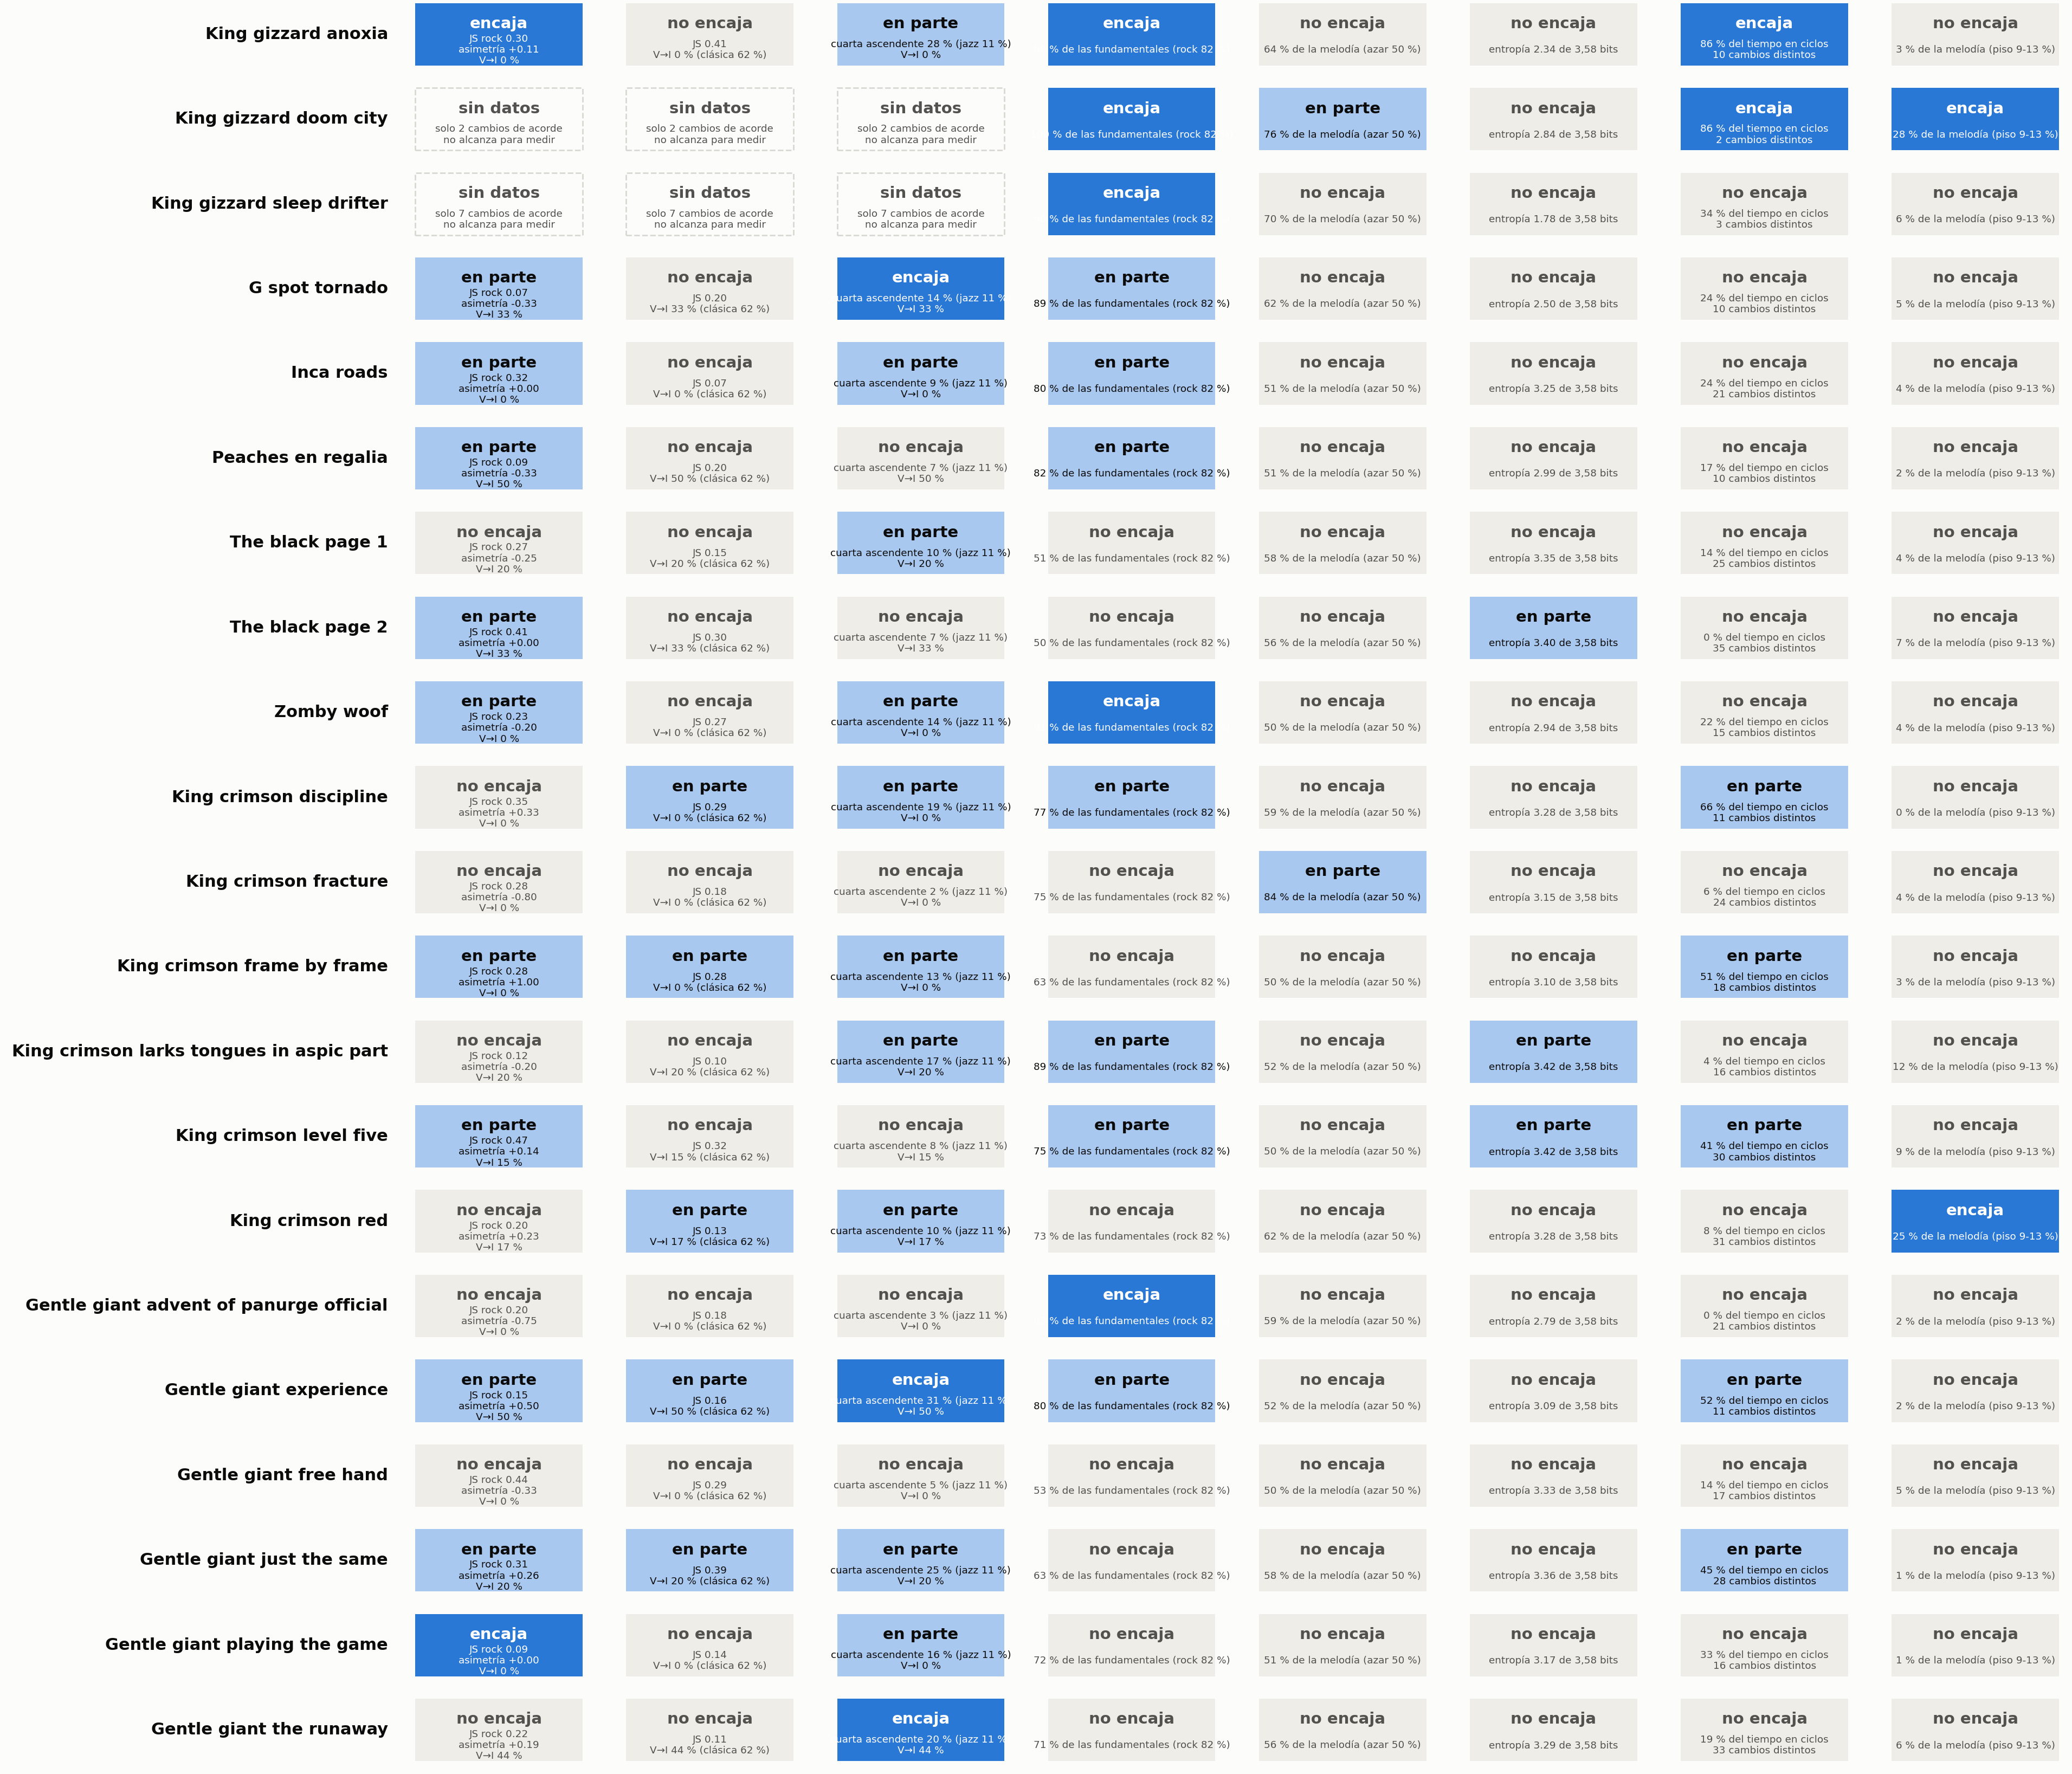
\includegraphics[width=\textwidth,height=0.78\textheight,keepaspectratio]{g_veredictos_estilos_2.png}
  \caption{Pruebas de estilo con reglas, canciones 16--36; misma lectura que la figura~\ref{fig:g-veredictos1}.}\label{fig:g-veredictos2}
\end{figure}

\section{Melodía}

La figura~\ref{fig:g-uso} amplía la figura~\ref{fig:uso} a las 36 canciones, y las figuras~\ref{fig:g-escalas1} y~\ref{fig:g-escalas2} muestran la escala de cada una.

\begin{figure}[!htbp]
  \centering
  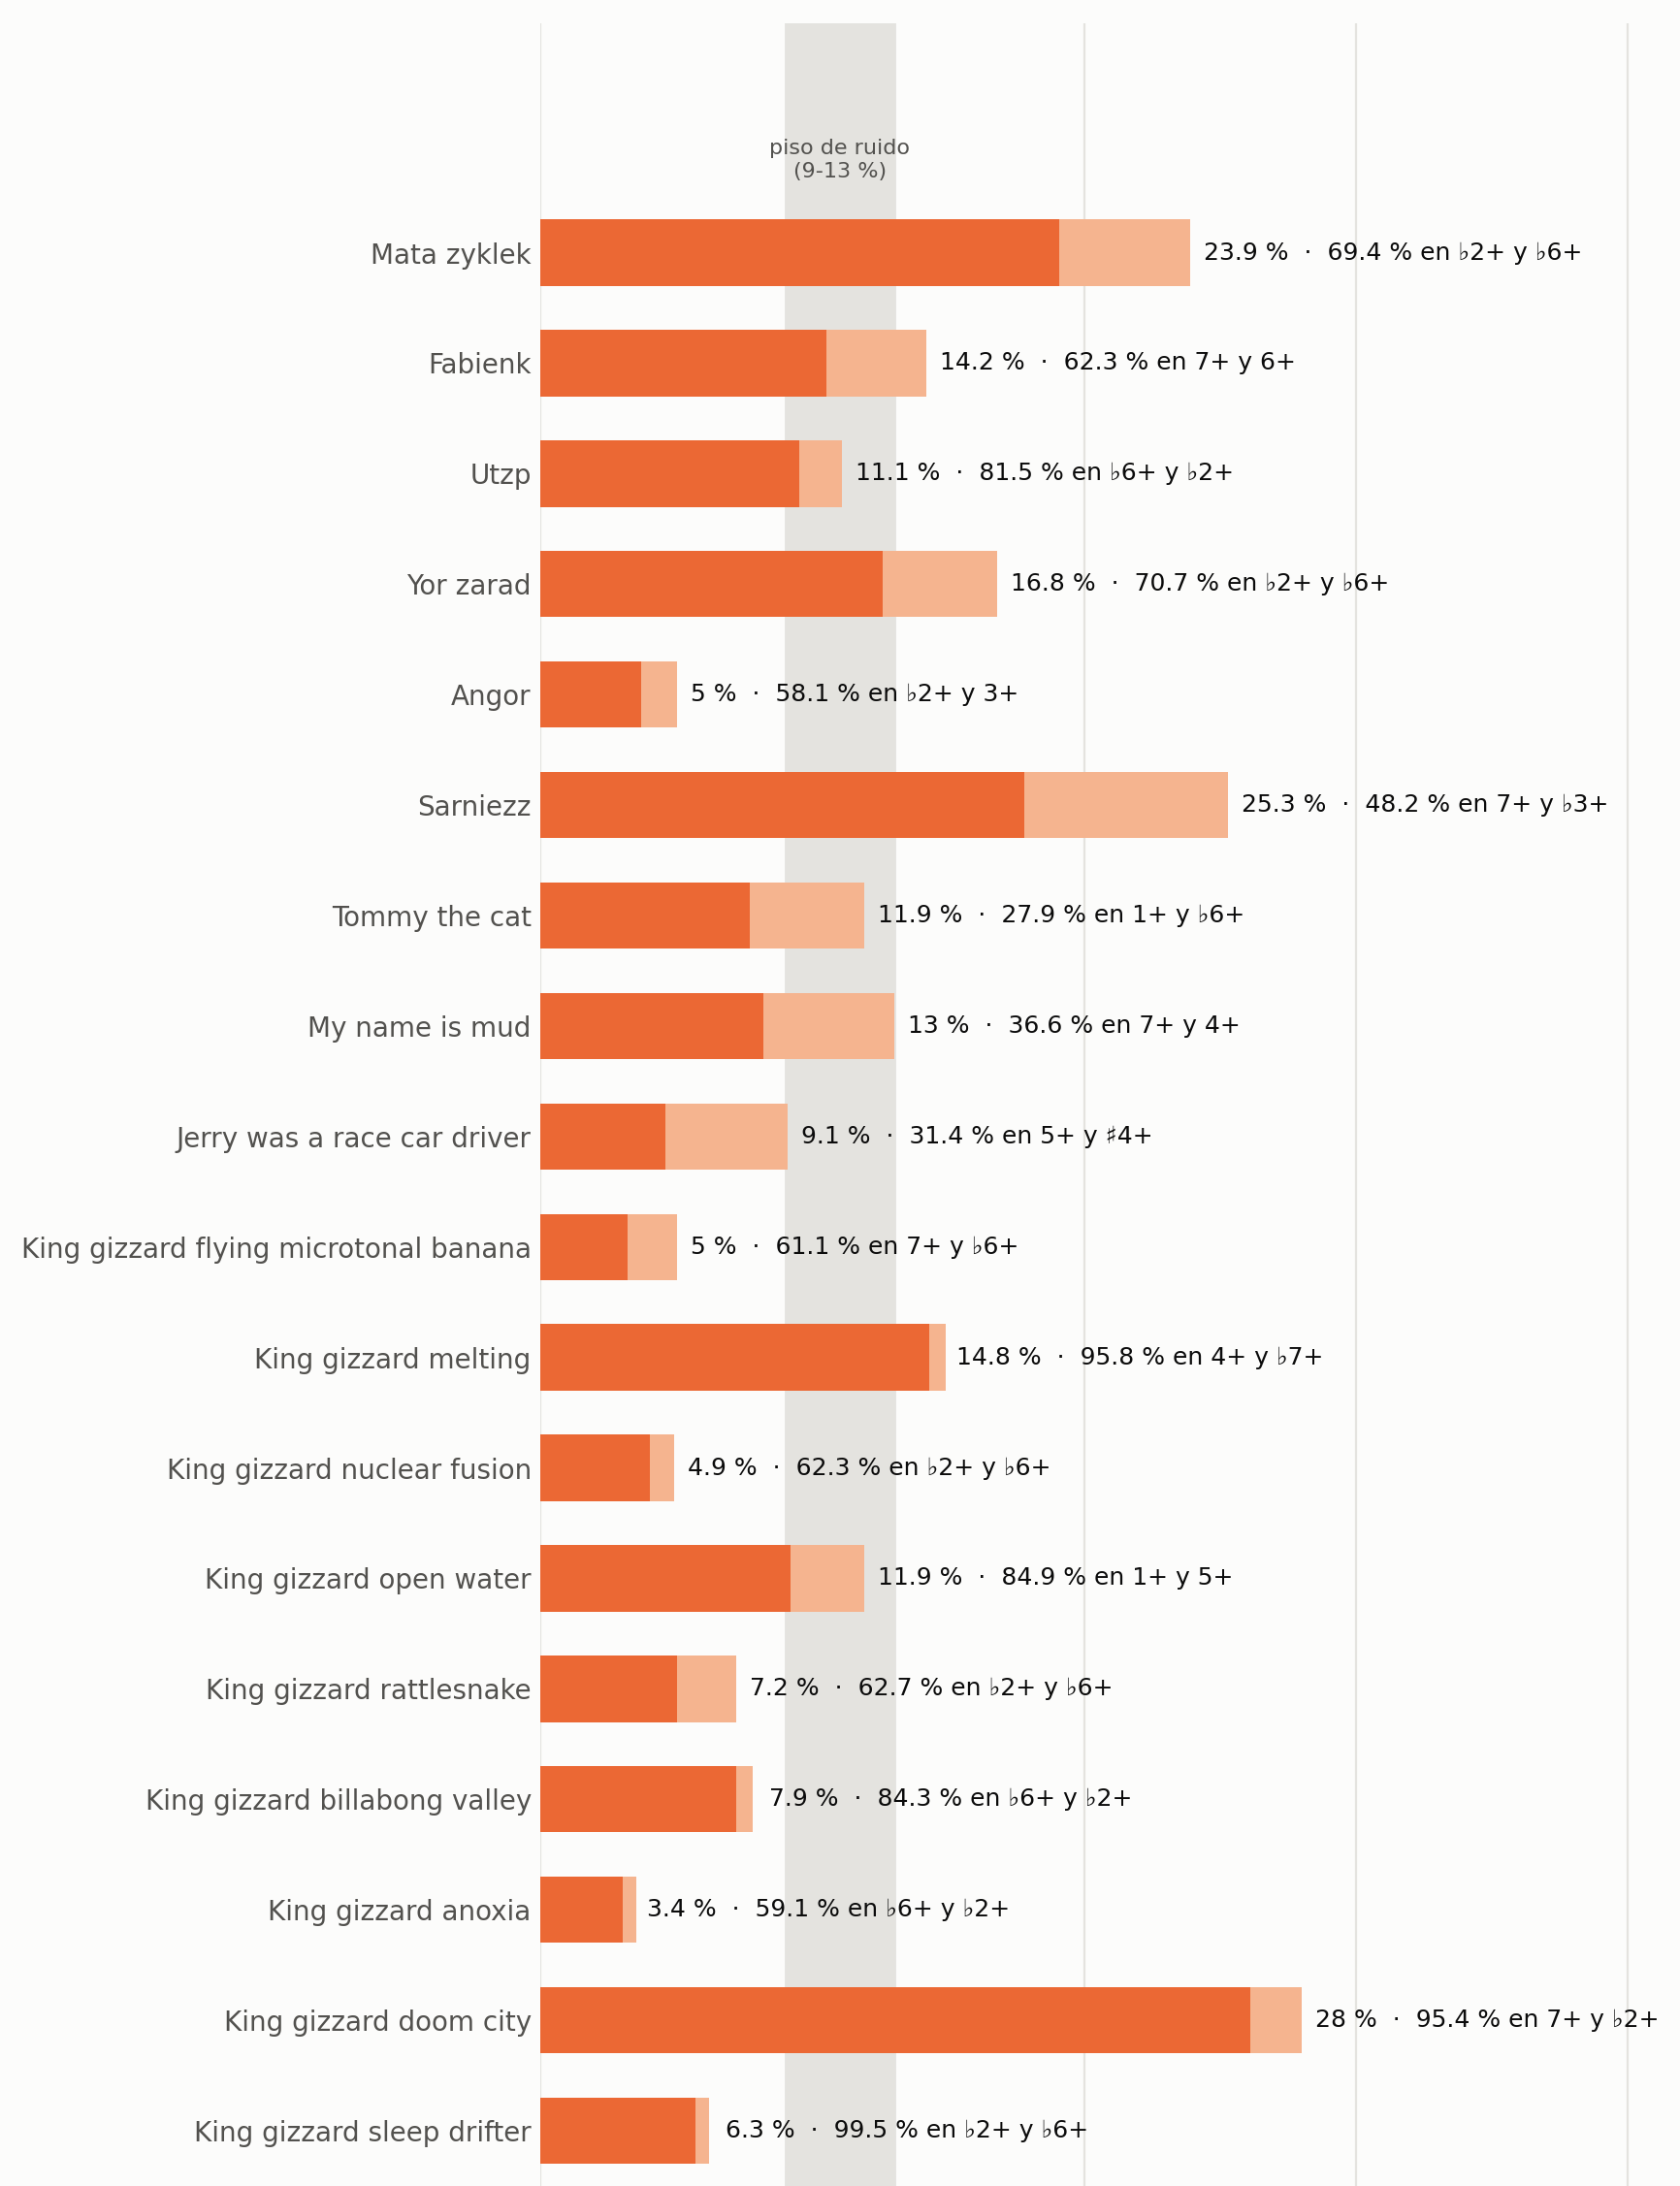
\includegraphics[width=0.495\textwidth]{g_microtonal_uso_a.png}\hfill
  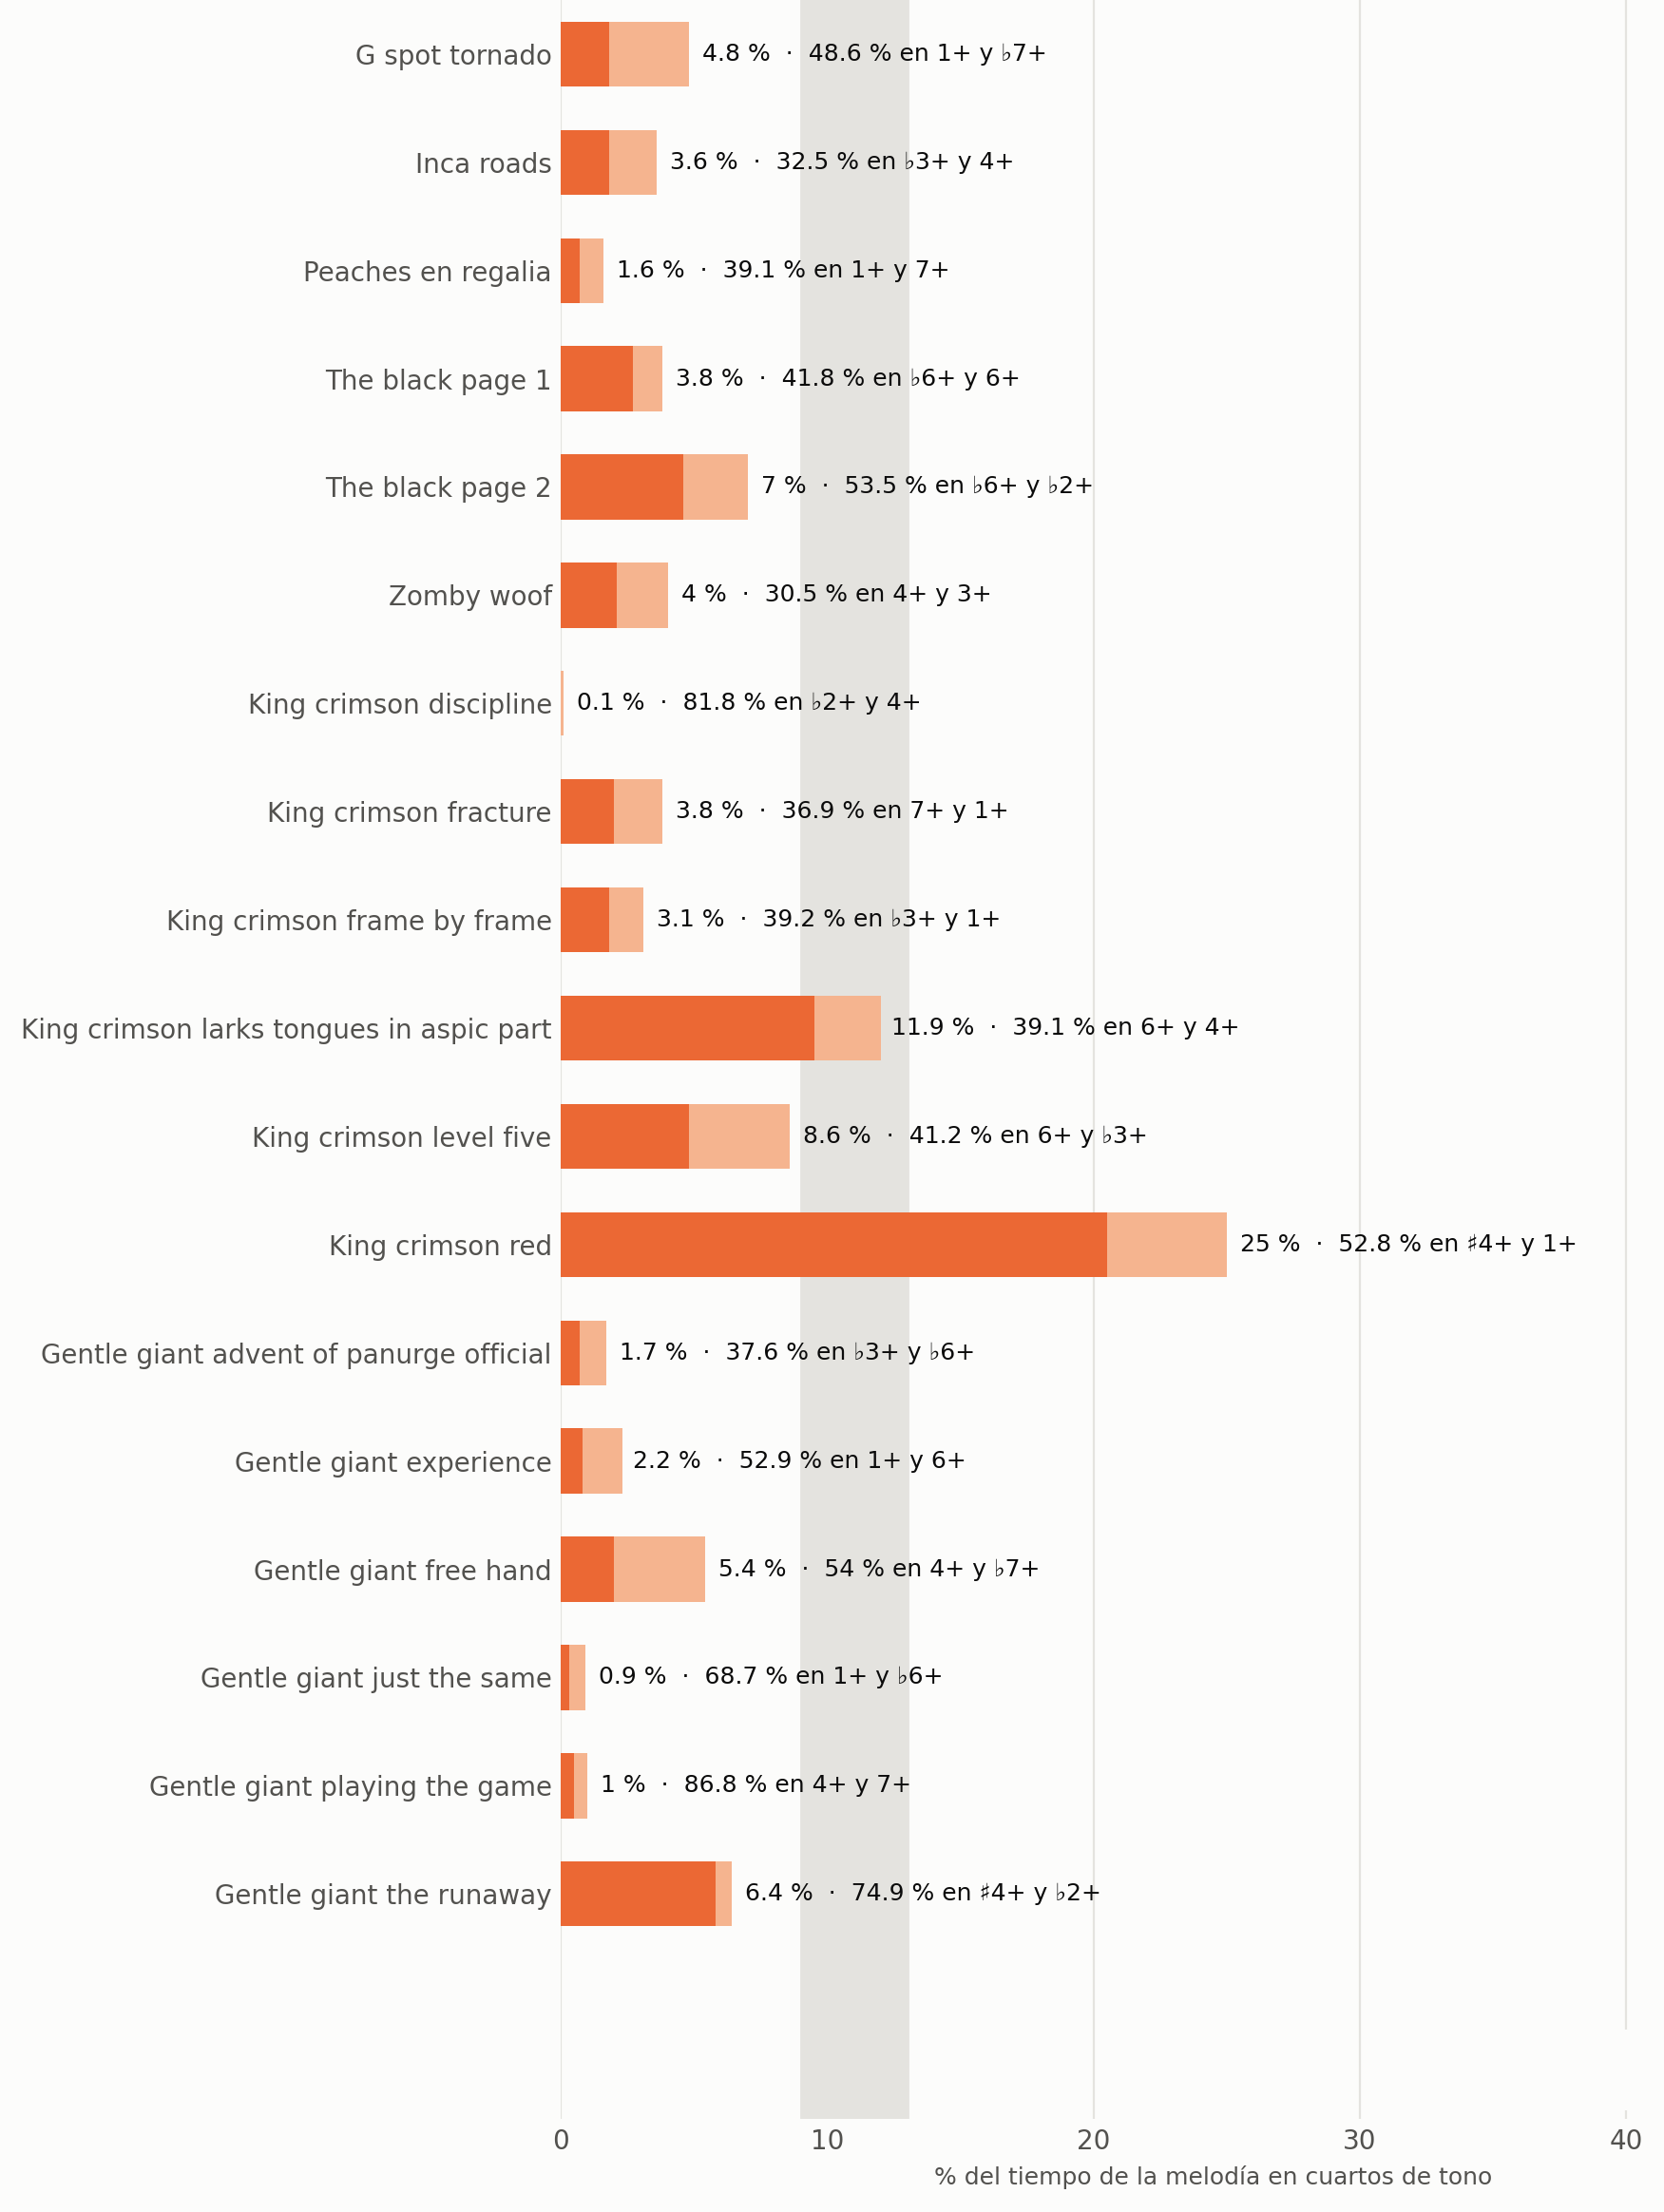
\includegraphics[width=0.495\textwidth]{g_microtonal_uso_b.png}
  \caption{Cuartos de tono en la melodía de las 36 canciones. Naranja oscuro: como grado; claro: como adorno; franja gris: piso de ruido (9--13\,\%). Junto a cada barra, el total y la fracción en los dos grados más usados. Las canciones siguen en la columna derecha.}\label{fig:g-uso}
\end{figure}

\begin{figure}[!htbp]
  \centering
  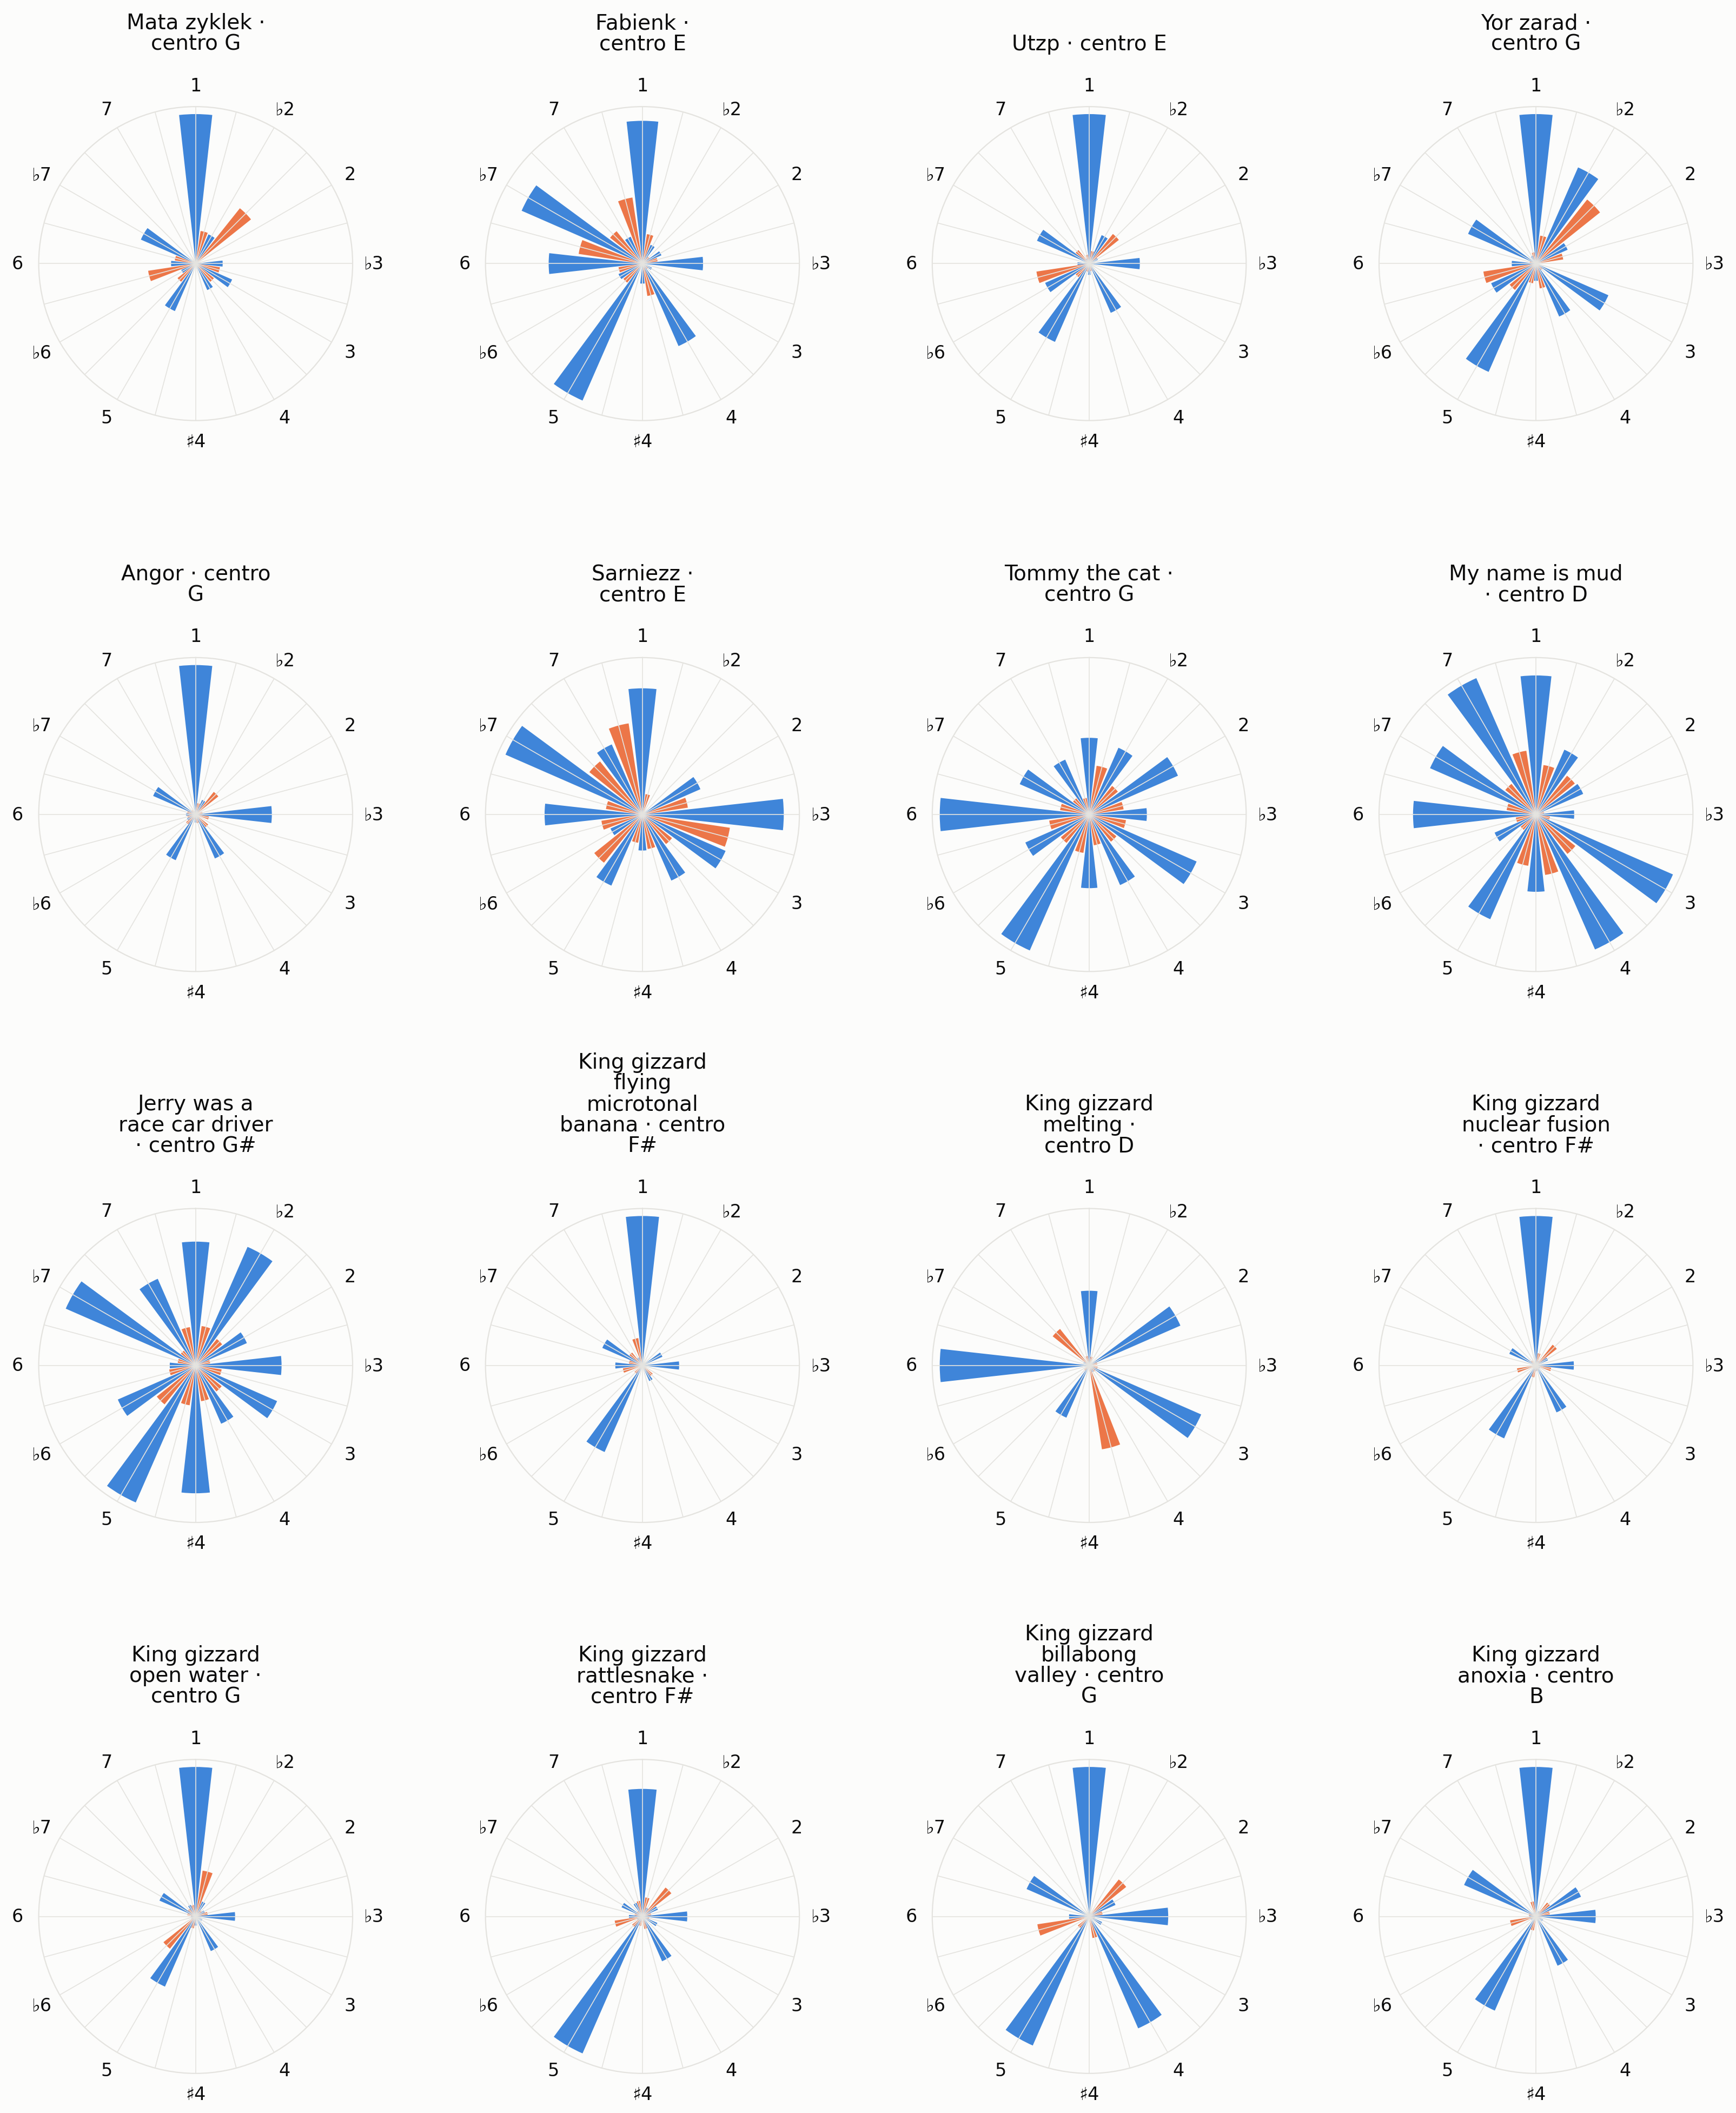
\includegraphics[width=\textwidth,height=0.78\textheight,keepaspectratio]{g_microtonal_escalas_1.png}
  \caption{Escala de cada canción en 24-EDO respecto de su centro (I). Largo del pétalo: tiempo en el grado; azul: grado regular; rojo: cuarto de tono.}\label{fig:g-escalas1}
\end{figure}

\begin{figure}[!htbp]
  \centering
  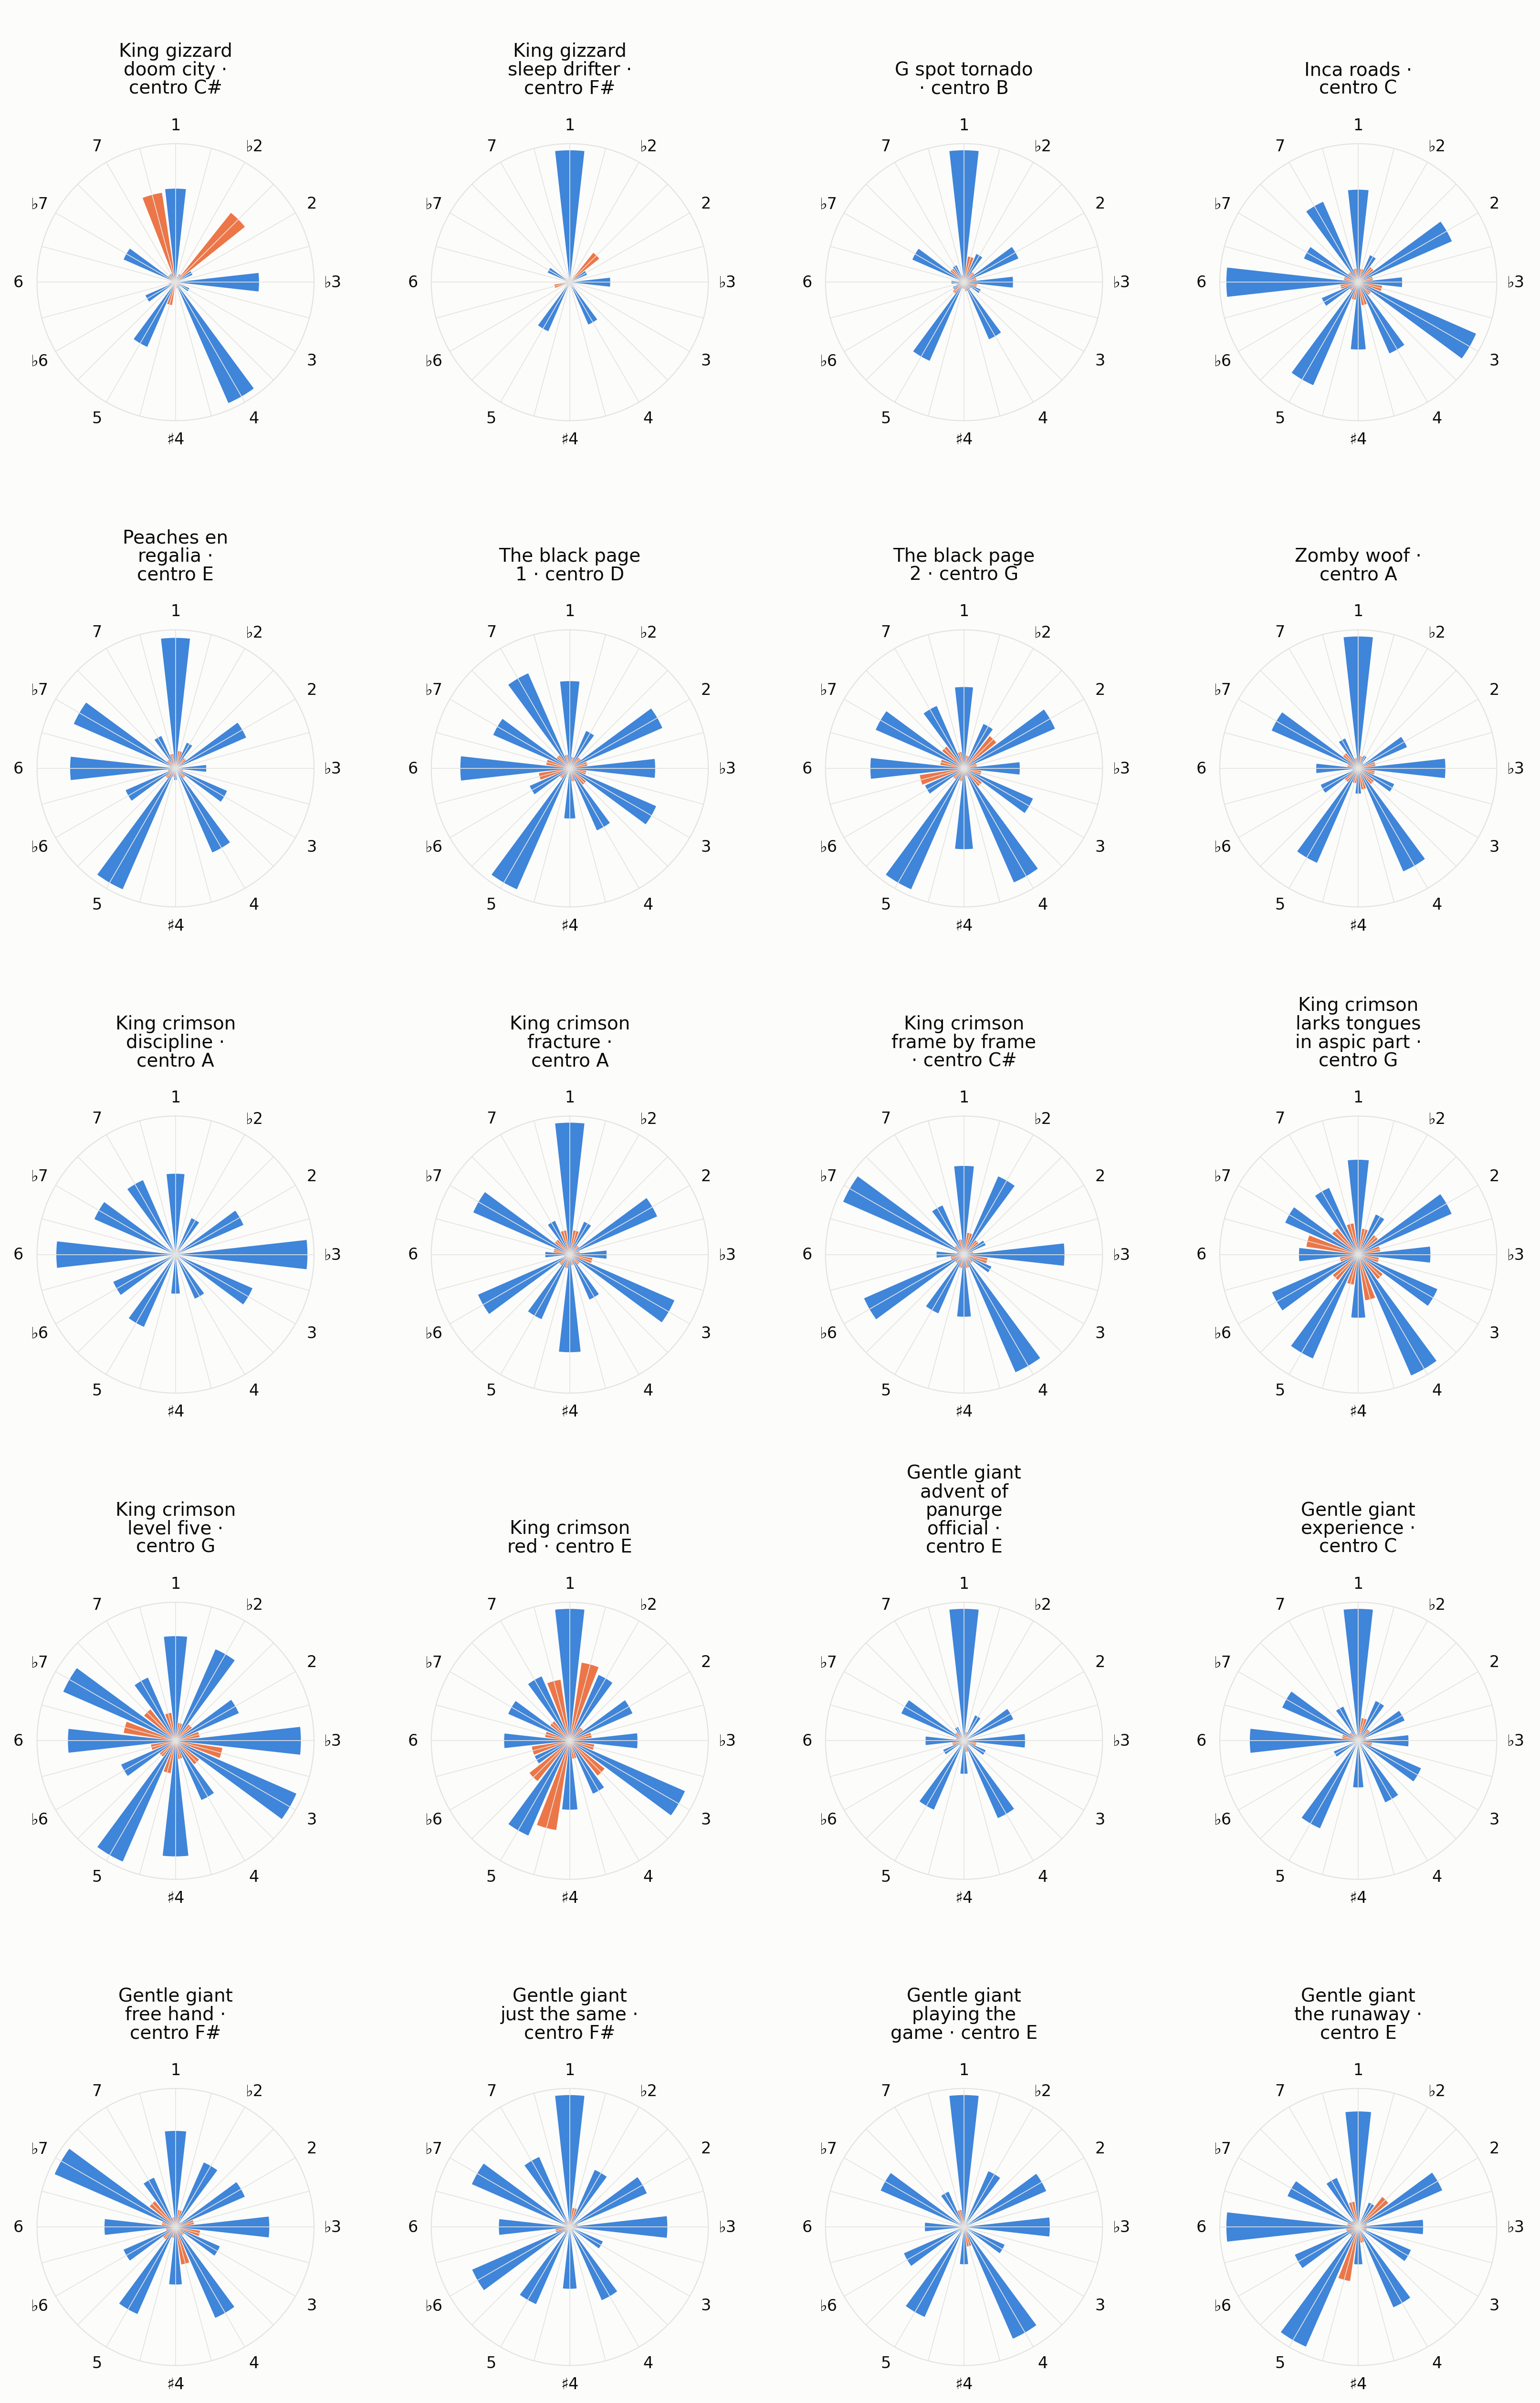
\includegraphics[width=\textwidth,height=0.78\textheight,keepaspectratio]{g_microtonal_escalas_2.png}
  \caption{Escala de cada canción en 24-EDO (II); misma lectura que la figura~\ref{fig:g-escalas1}.}\label{fig:g-escalas2}
\end{figure}

\section{Síntesis}

Las figuras~\ref{fig:g-bloques} y~\ref{fig:g-bloques-sintesis} dan el test por bloques completo (sección~\ref{sec:res-sintesis}).

\begin{figure}[!htbp]
  \centering
  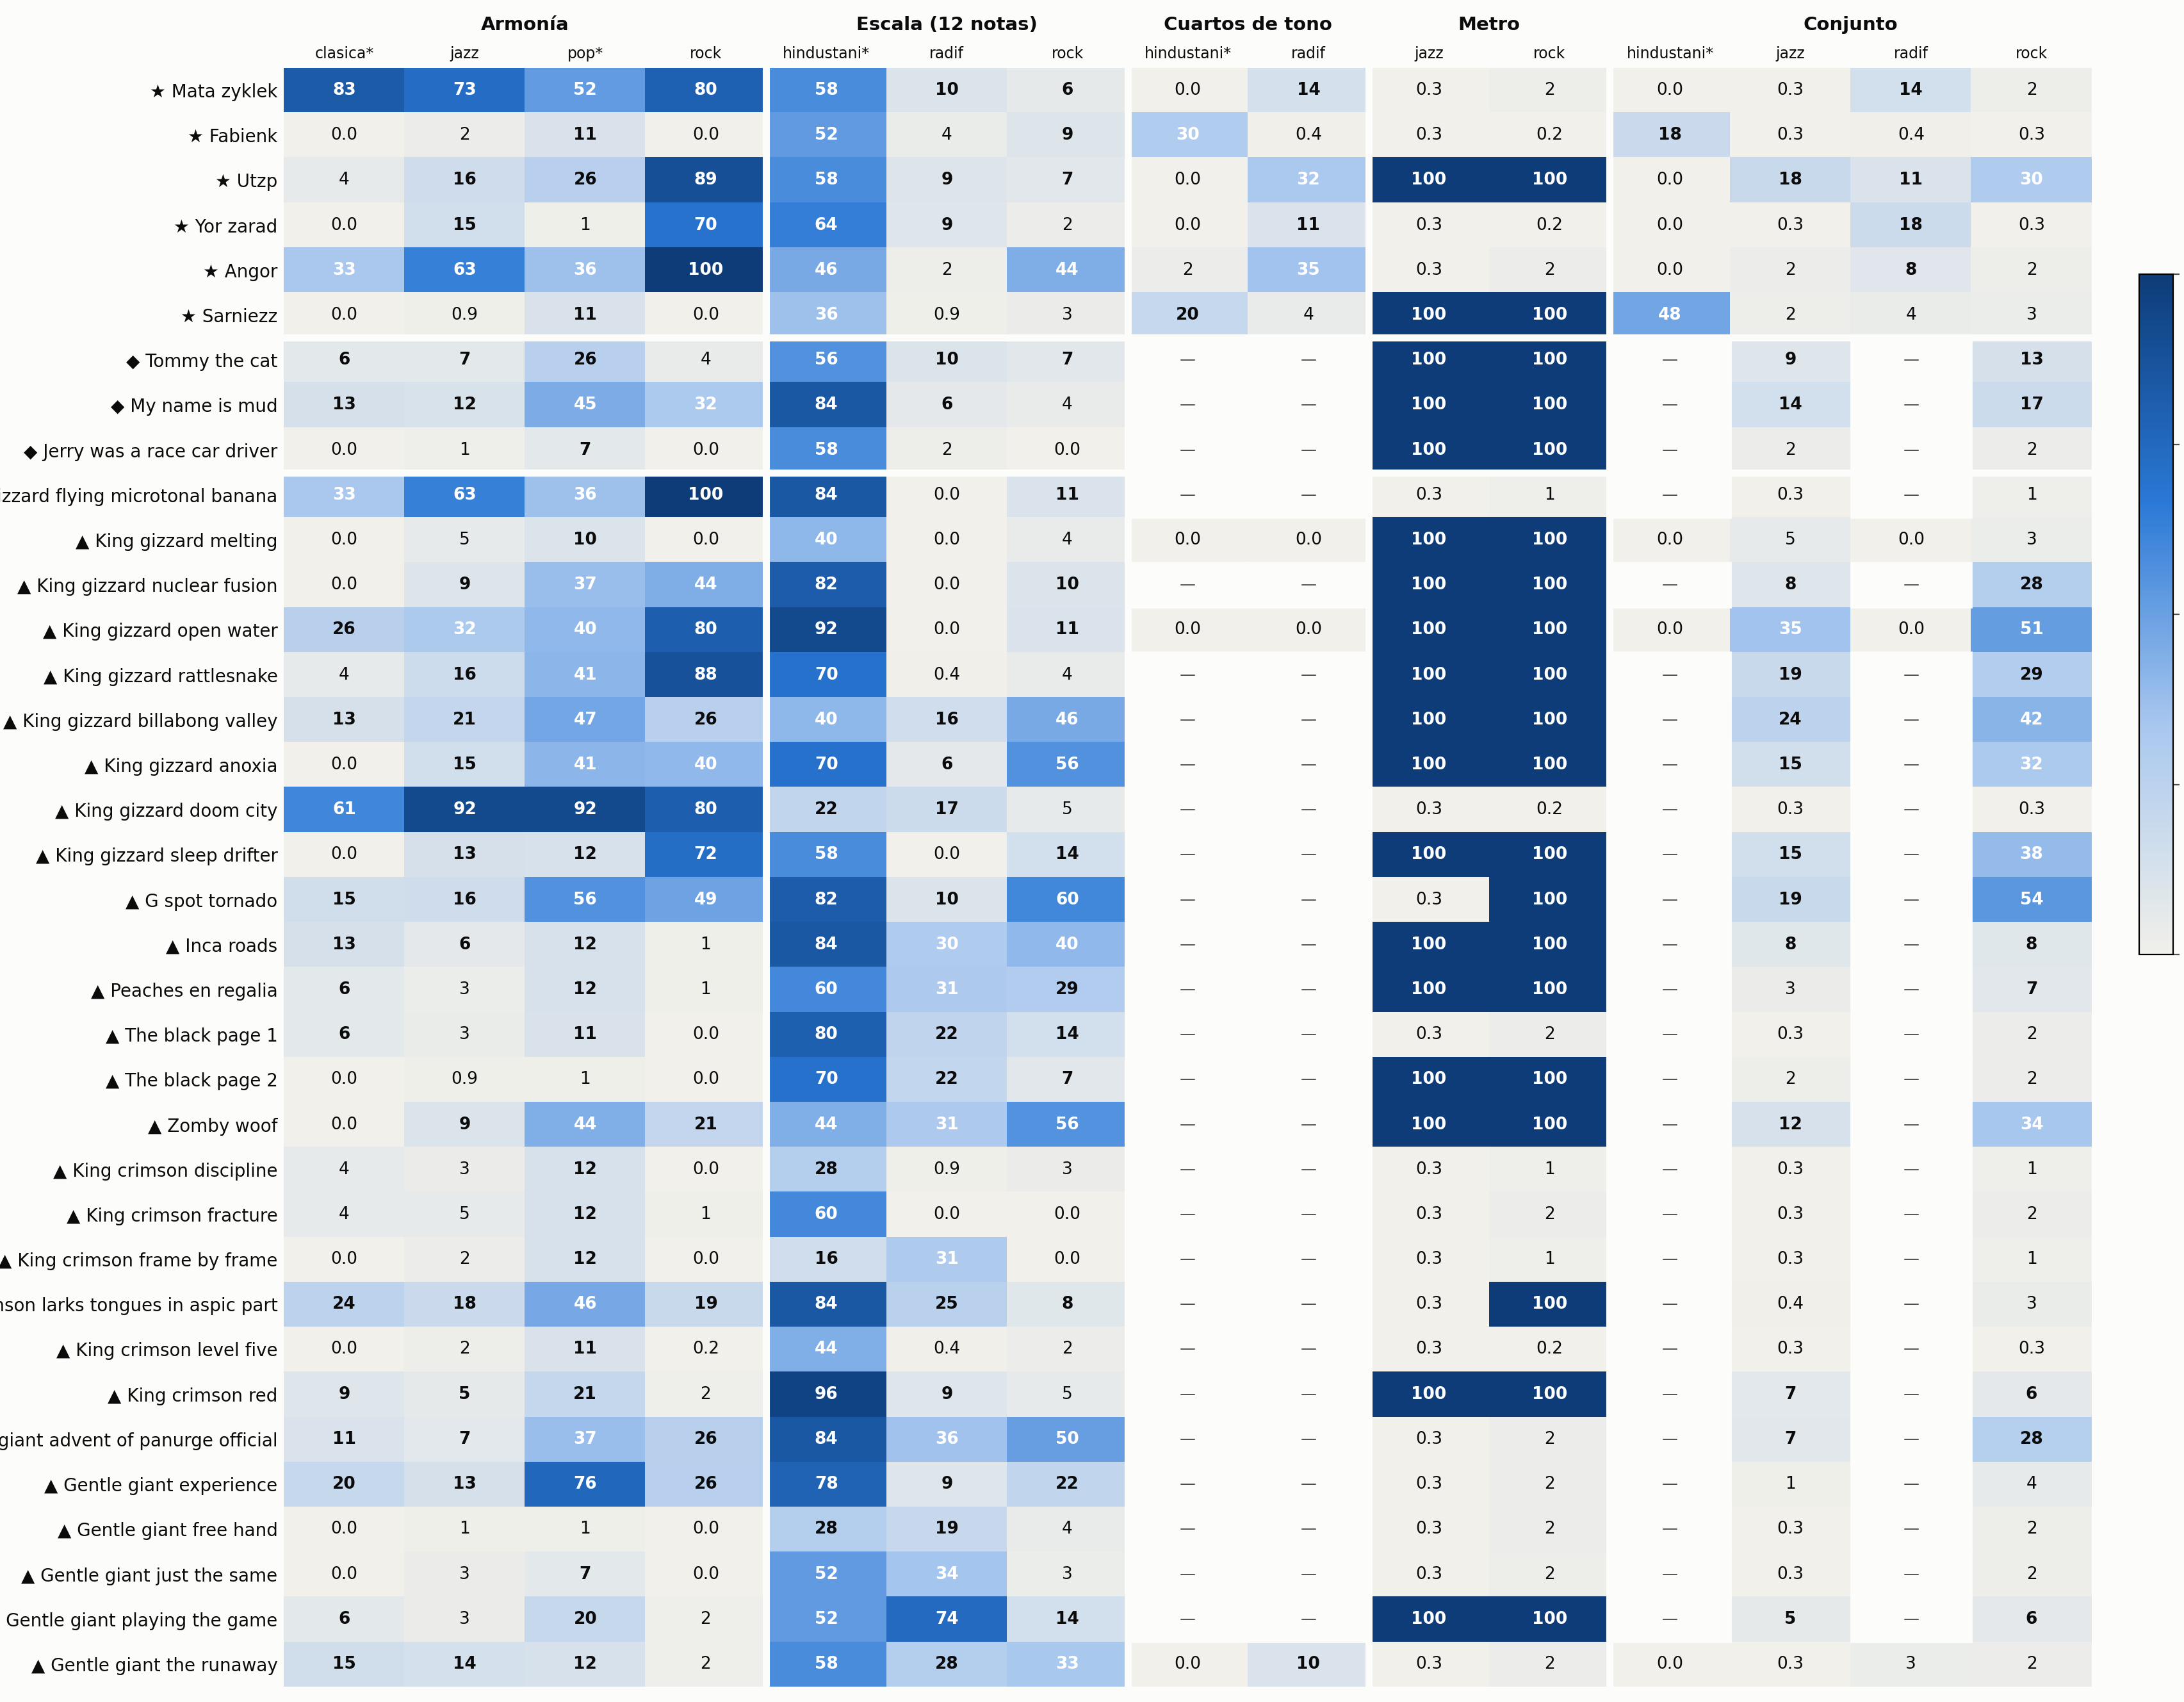
\includegraphics[width=\textwidth,height=0.78\textheight,keepaspectratio]{g_bloques.png}
  \caption{Test por bloques de las 36 canciones: percentil de cada canción en cada corpus y bloque (oscuro = típico). Símbolos: círculo, la banda; rombo, Primus; triángulo, repertorio comparado. Columnas agrupadas por bloque (armonía, escala en 12 notas, cuartos de tono, metro y conjunto). Asterisco: corpus de menos de 100 piezas (los tamaños están en la tabla~\ref{tab:corpus}); raya: sin datos. Las piezas de corpus pasan por el error de la herramienta ($\varepsilon = 0.11$ en altura, $\eta = 0.07$ en metro).}\label{fig:g-bloques}
\end{figure}

\begin{figure}[!htbp]
  \centering
  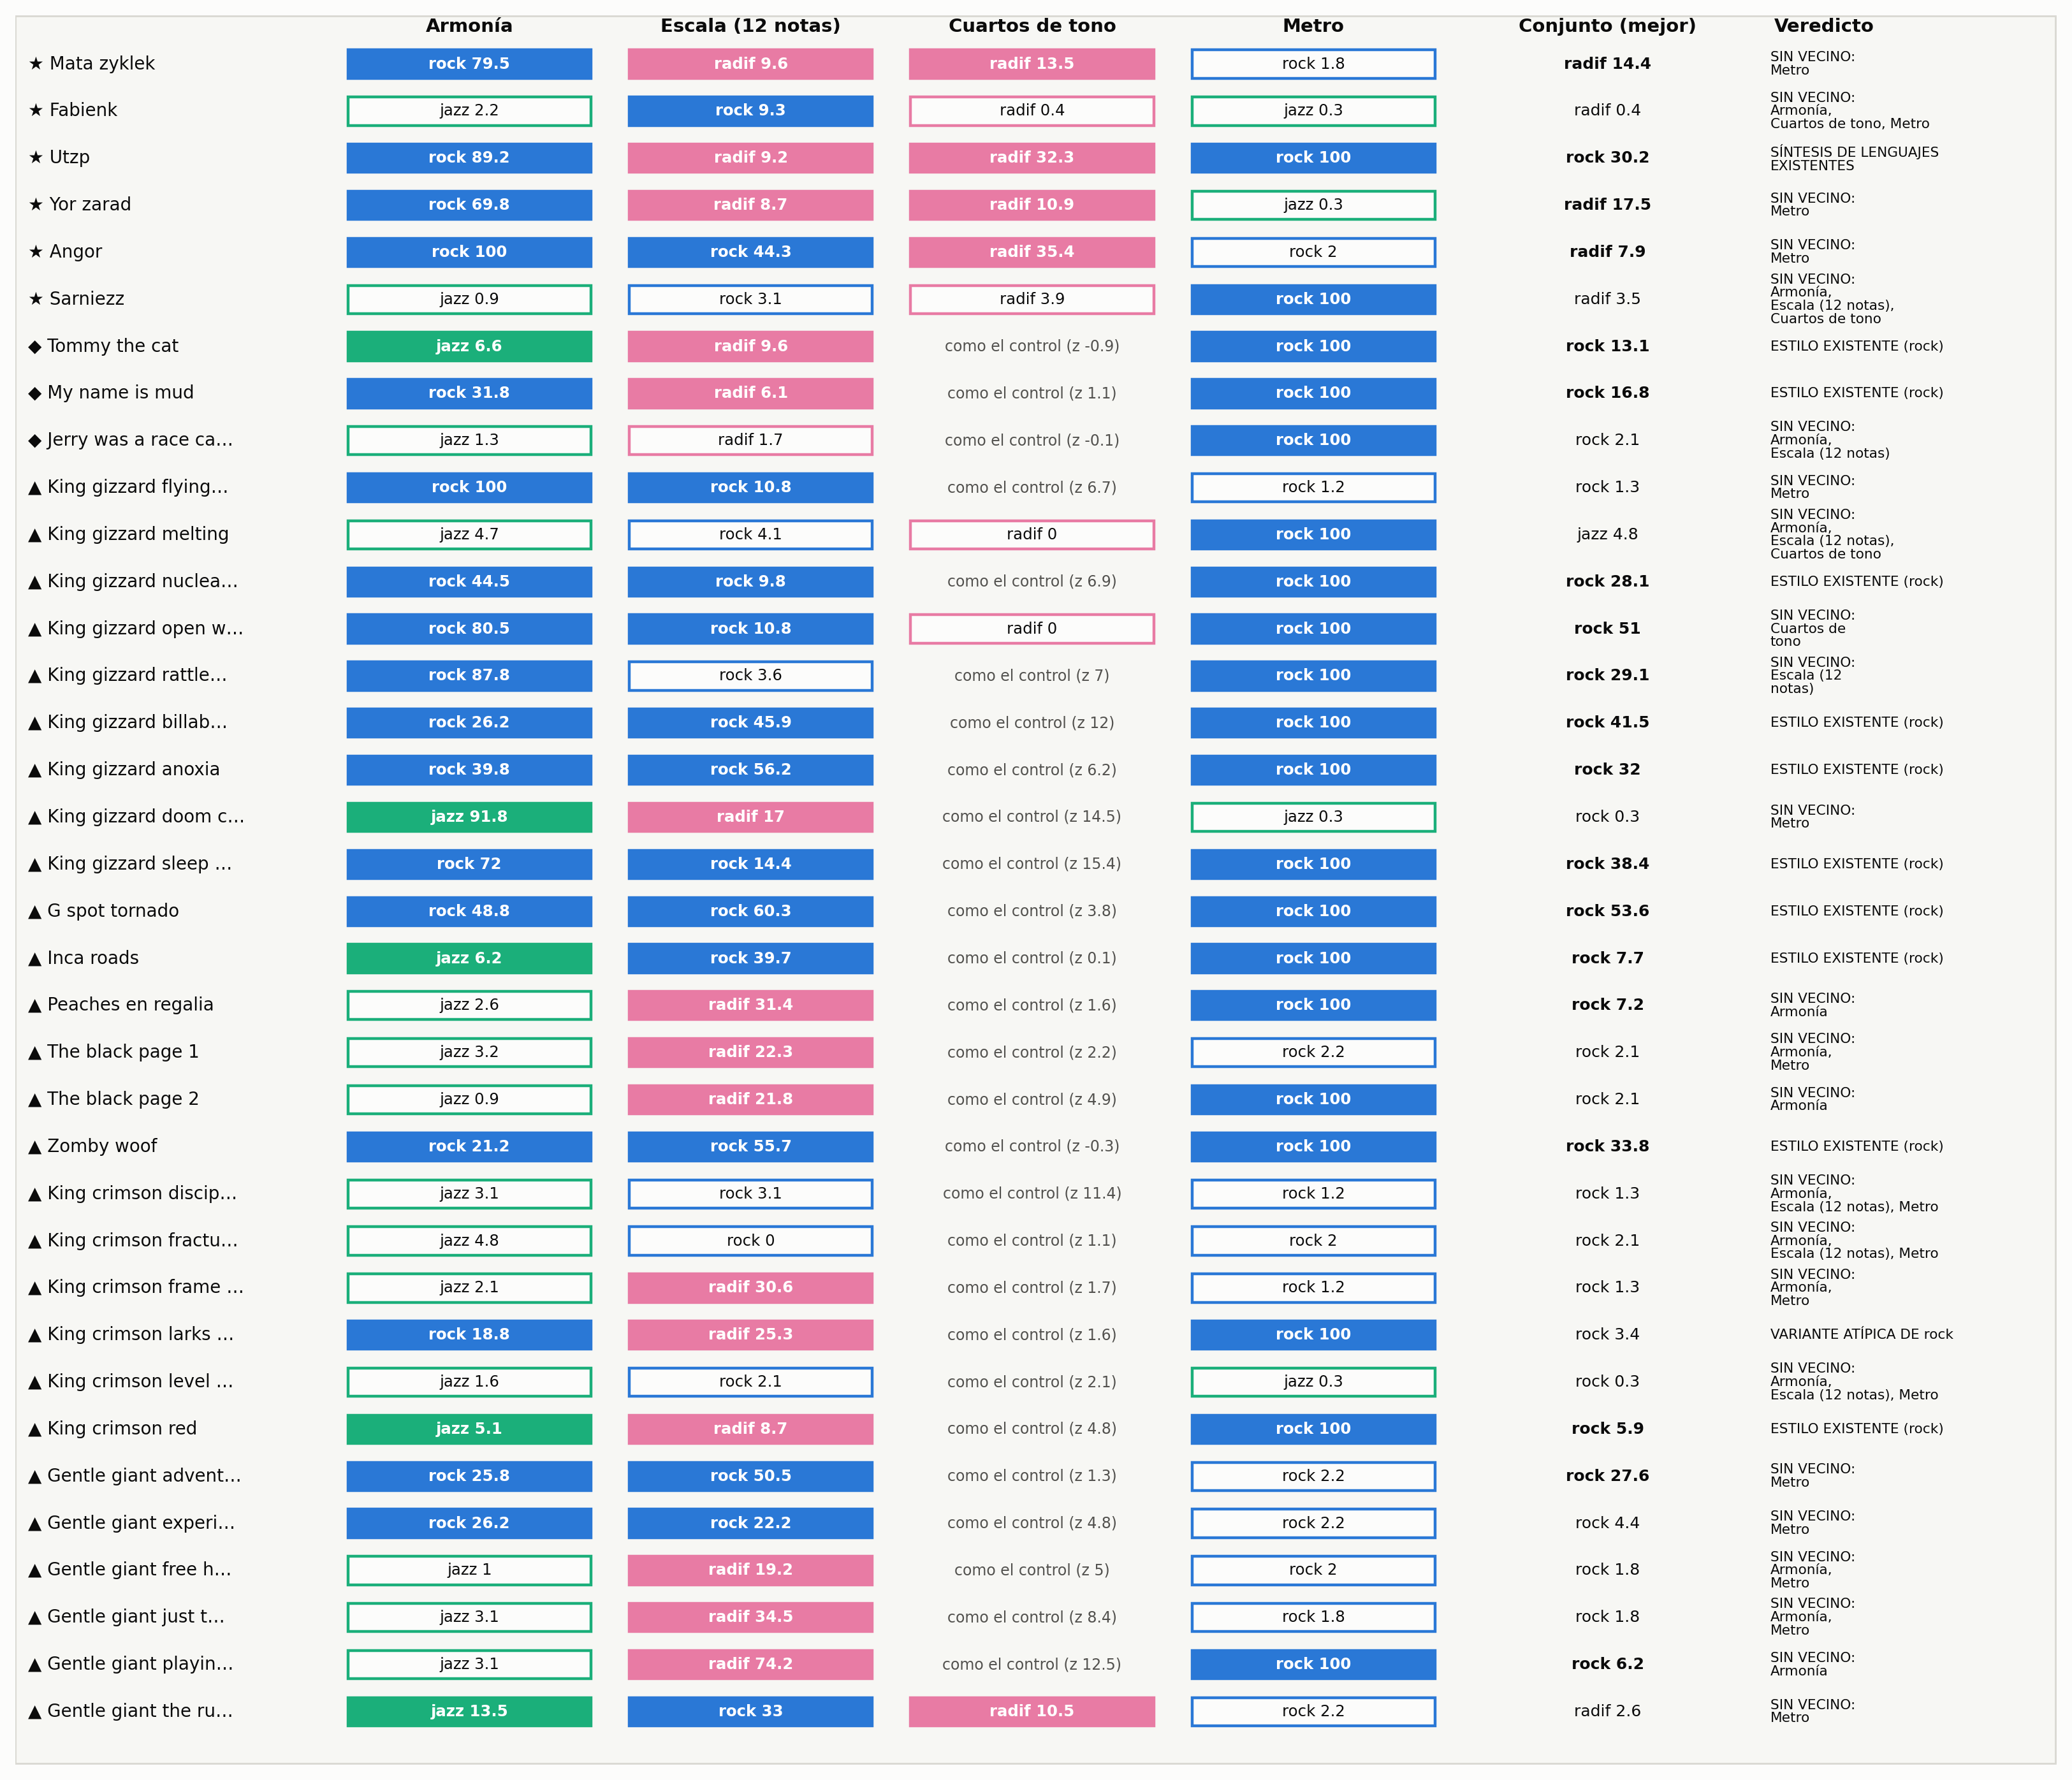
\includegraphics[width=\textwidth]{g_bloques_sintesis.png}
  \caption{Corpus más probable por bloque y veredicto de cada canción. Color: naranja, clásica; verde, jazz; rosa, microtonal; azul, rock o pop. Casilla vacía: hay datos, pero el percentil queda bajo el umbral; raya: sin datos comparables; «como el control»: concentración que no supera la de Primus. En cuartos de tono, la concentración de la banda se compara con la de Primus ($32 \pm 4$\,\%); si no la supera, no se lee como escala microtonal.}\label{fig:g-bloques-sintesis}
\end{figure}

\section{Métricas estructurales}

Las figuras~\ref{fig:tarjetas1} y~\ref{fig:tarjetas2} comparan las métricas crudas de las tarjetas para las 36
canciones (sección~\ref{sec:repertorios}).

\begin{figure}[!htbp]
  \centering
  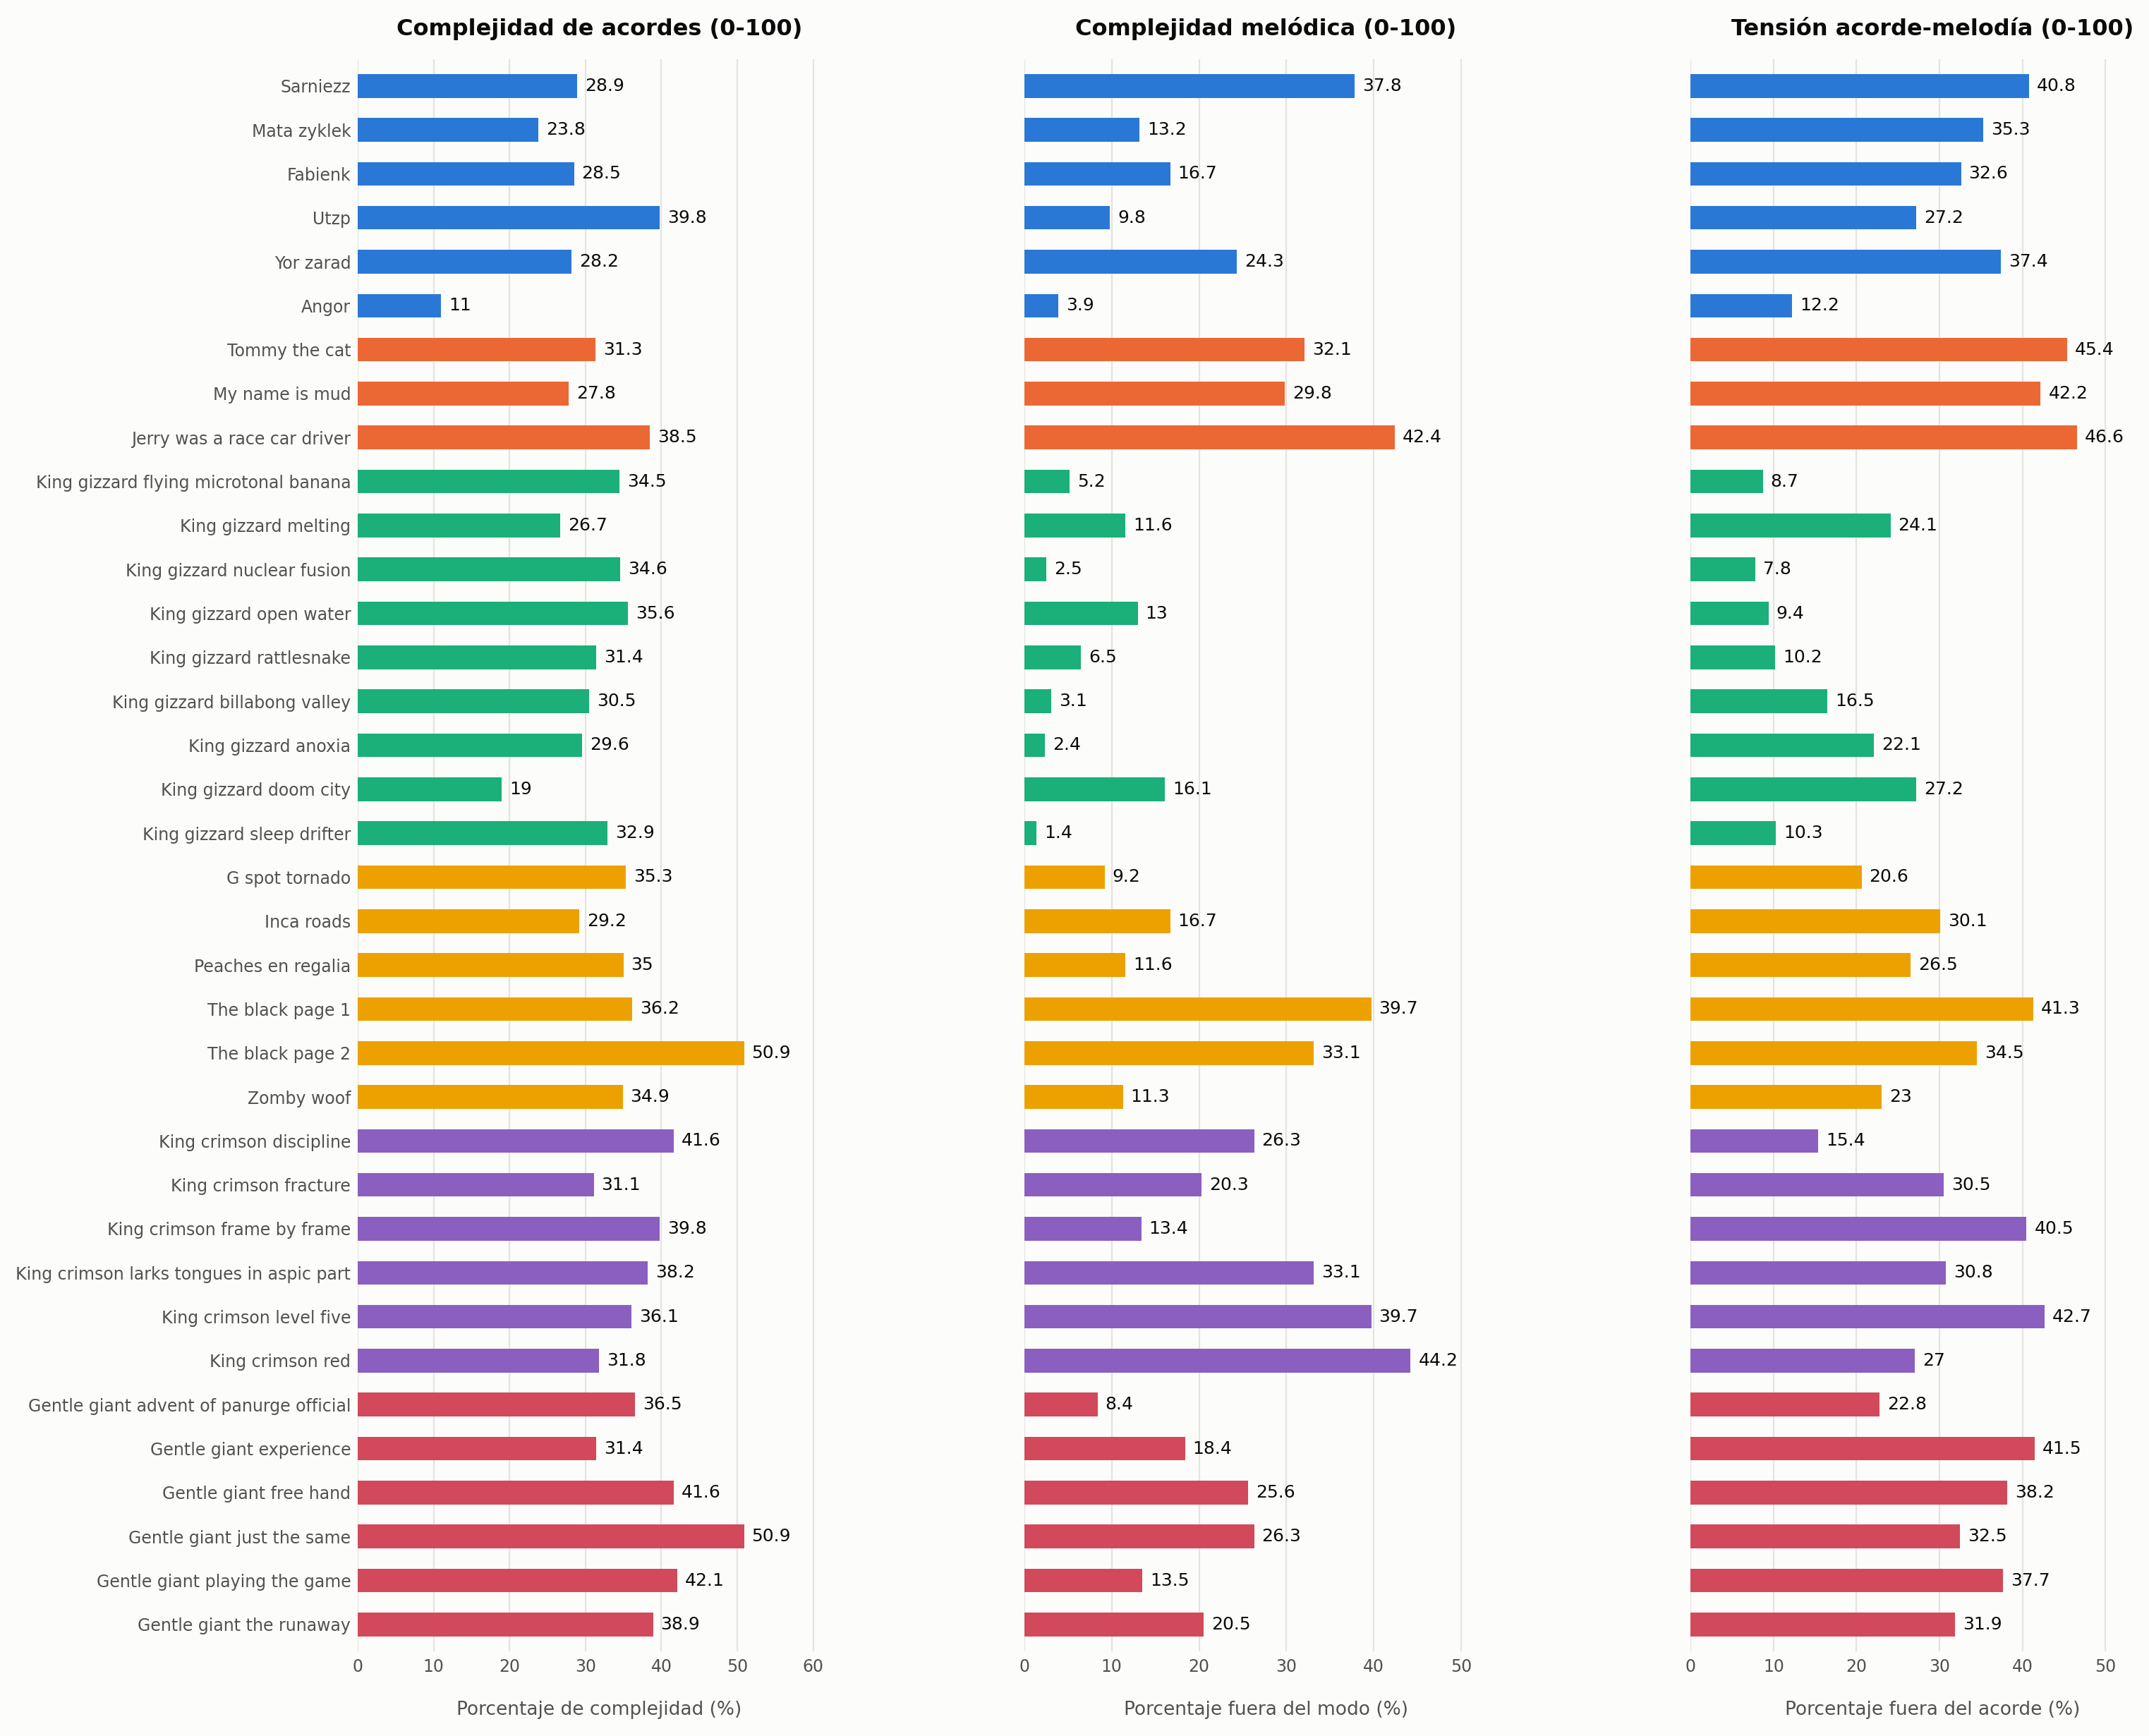
\includegraphics[width=\textwidth,height=0.78\textheight,keepaspectratio]{g_tarjetas_1.png}
  \caption{Métricas crudas de las 36 canciones (I): complejidad de acordes, complejidad melódica y tensión acorde-melodía (0--100). Color por artista: azul, la banda; naranja, Primus; verde, King Gizzard; amarillo, Zappa; violeta, King Crimson; rojo, Gentle Giant.}\label{fig:tarjetas1}
\end{figure}

\begin{figure}[!htbp]
  \centering
  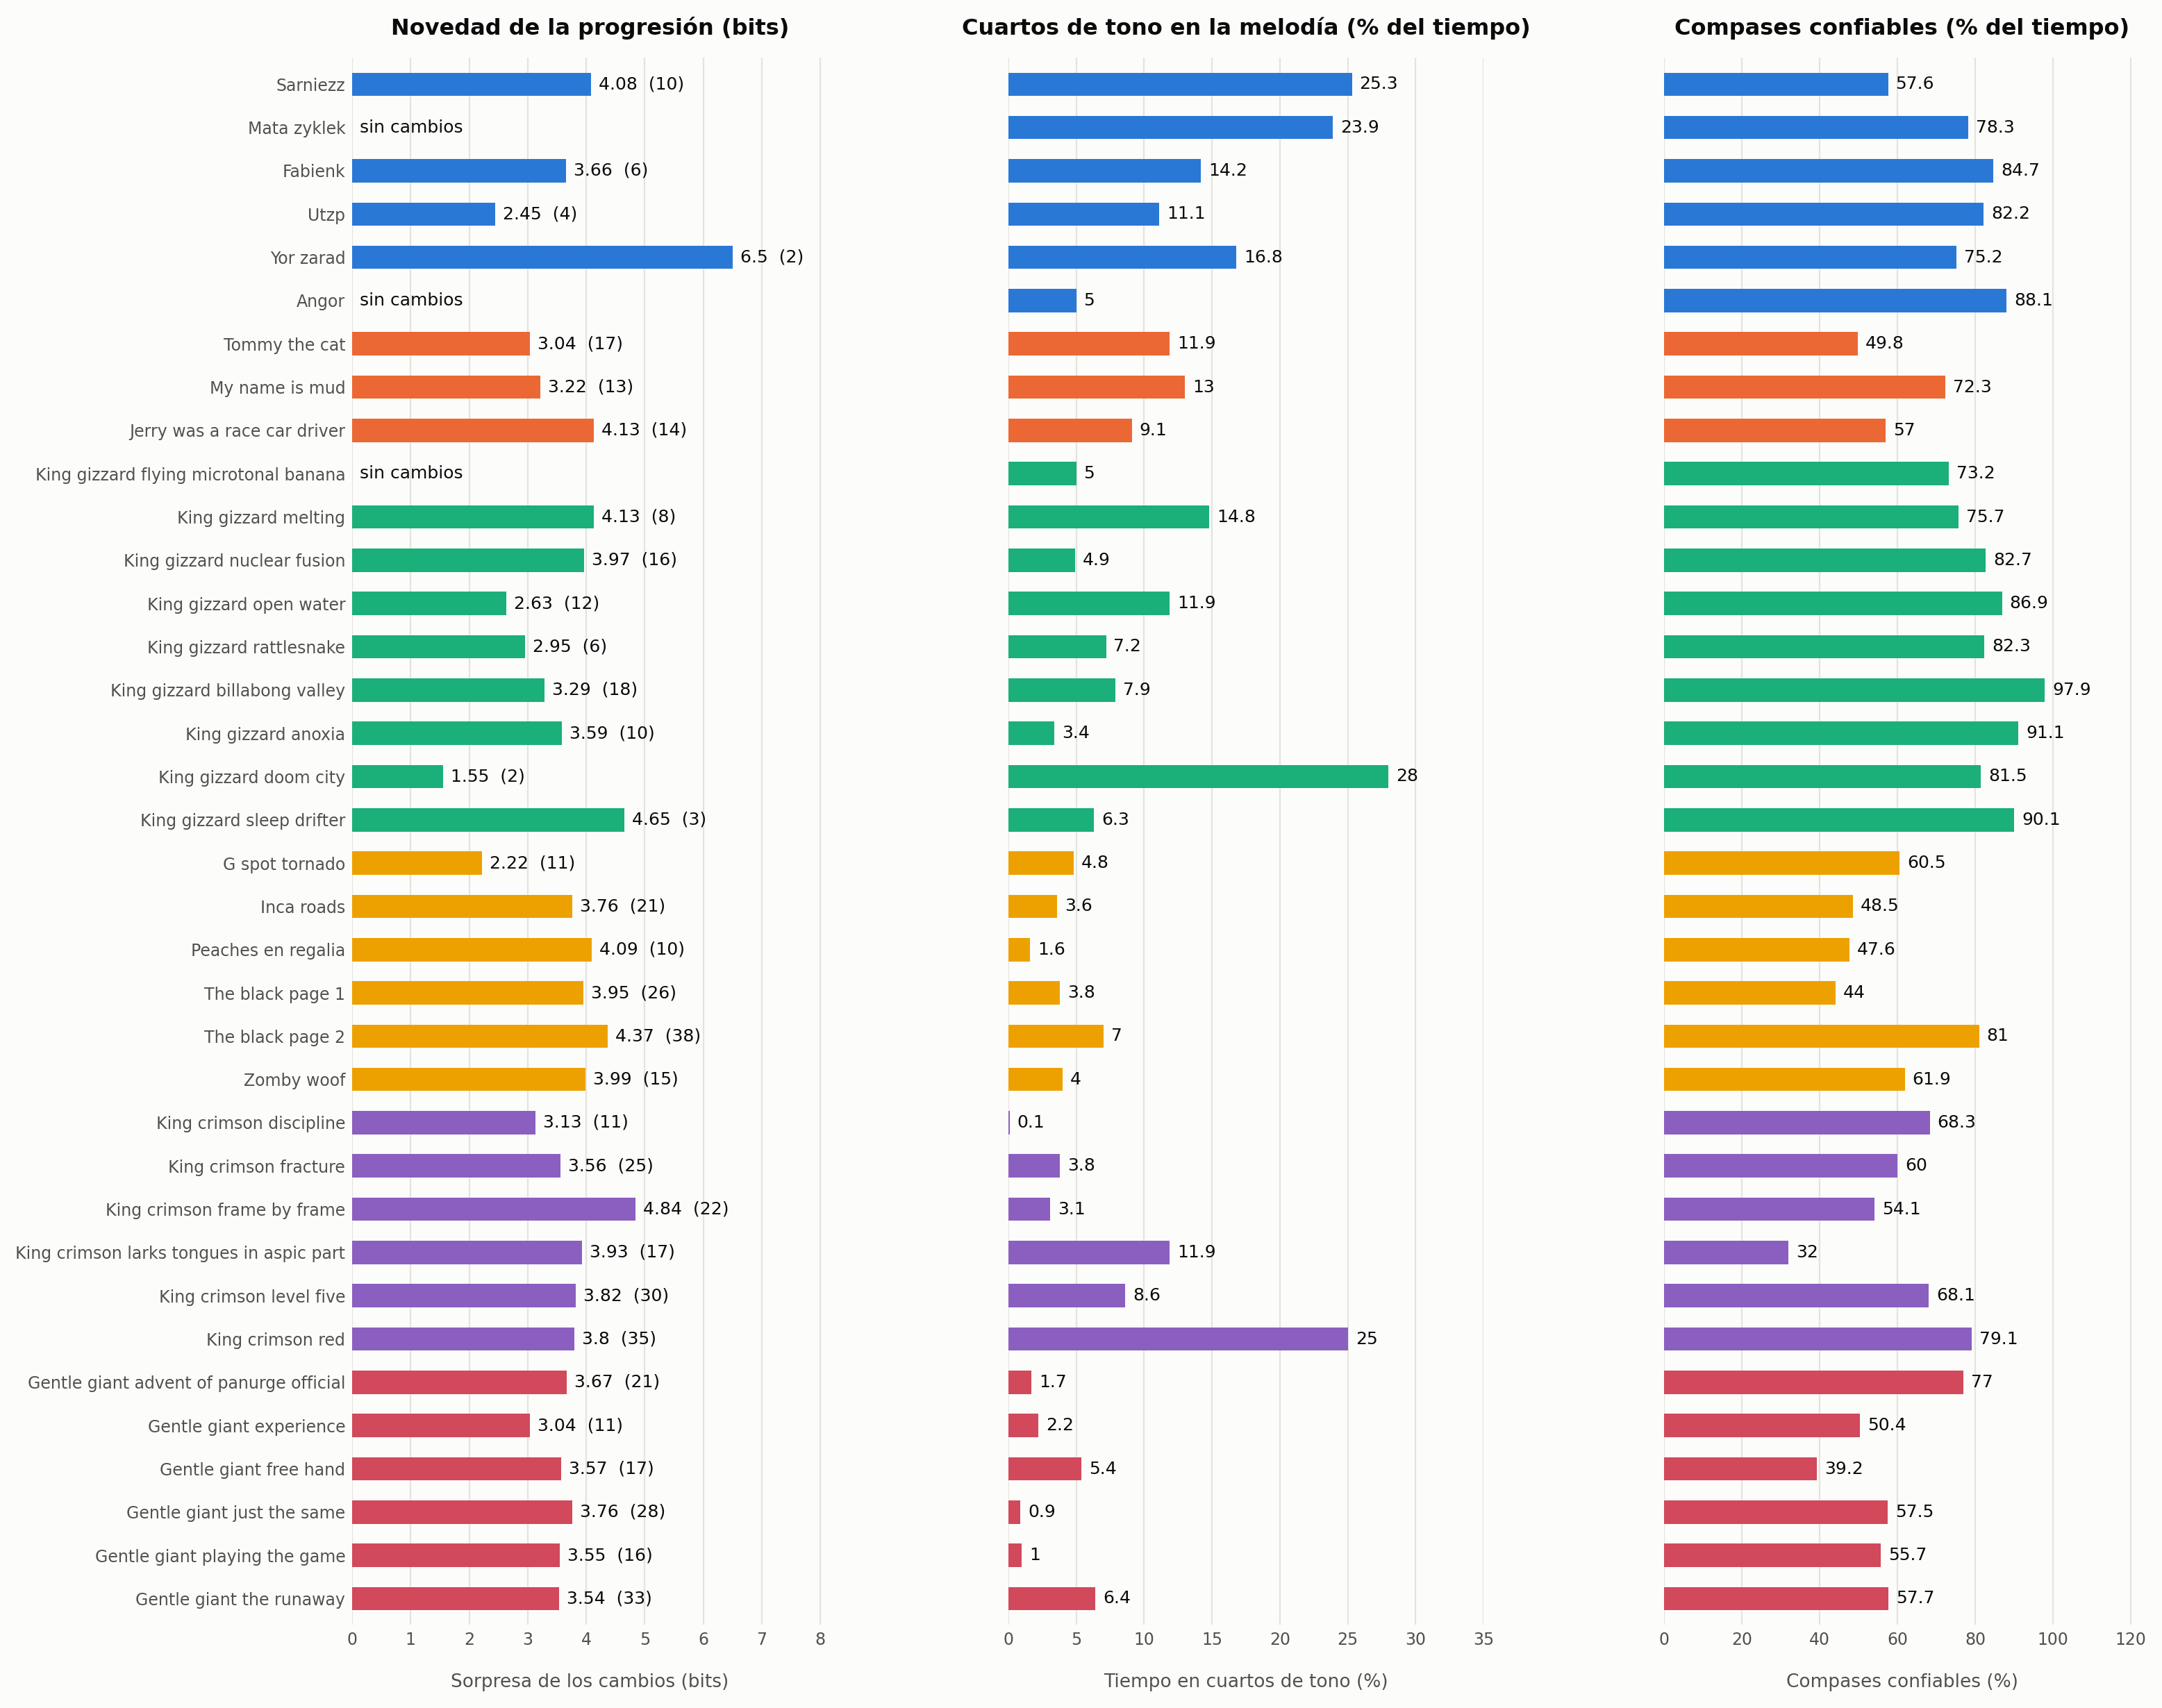
\includegraphics[width=\textwidth,height=0.78\textheight,keepaspectratio]{g_tarjetas_2.png}
  \caption{Métricas crudas (II): novedad de la progresión en bits (entre paréntesis, cambios distintos; con menos de 5 es poco estable), cuartos de tono en la melodía y compases confiables (\% del tiempo). Mismos colores que la figura~\ref{fig:tarjetas1}.}
  \label{fig:tarjetas2}
\end{figure}

\section{Radares de estilo (primera versión)}

Los radares de la figura~\ref{fig:radar-mata} (Mata Zyklek, en el capítulo~\ref{cap:metodologia}) y de las
figuras~\ref{fig:radar-fab-sar} y~\ref{fig:radar-yor-utzp} son de la versión del 15 de noviembre de 2026, anterior
al test por bloques; Angor no tenía todavía corrida en esa versión. Se incluyen como registro del método, no como
resultado.

\begin{figure}[!htbp]
  \centering
  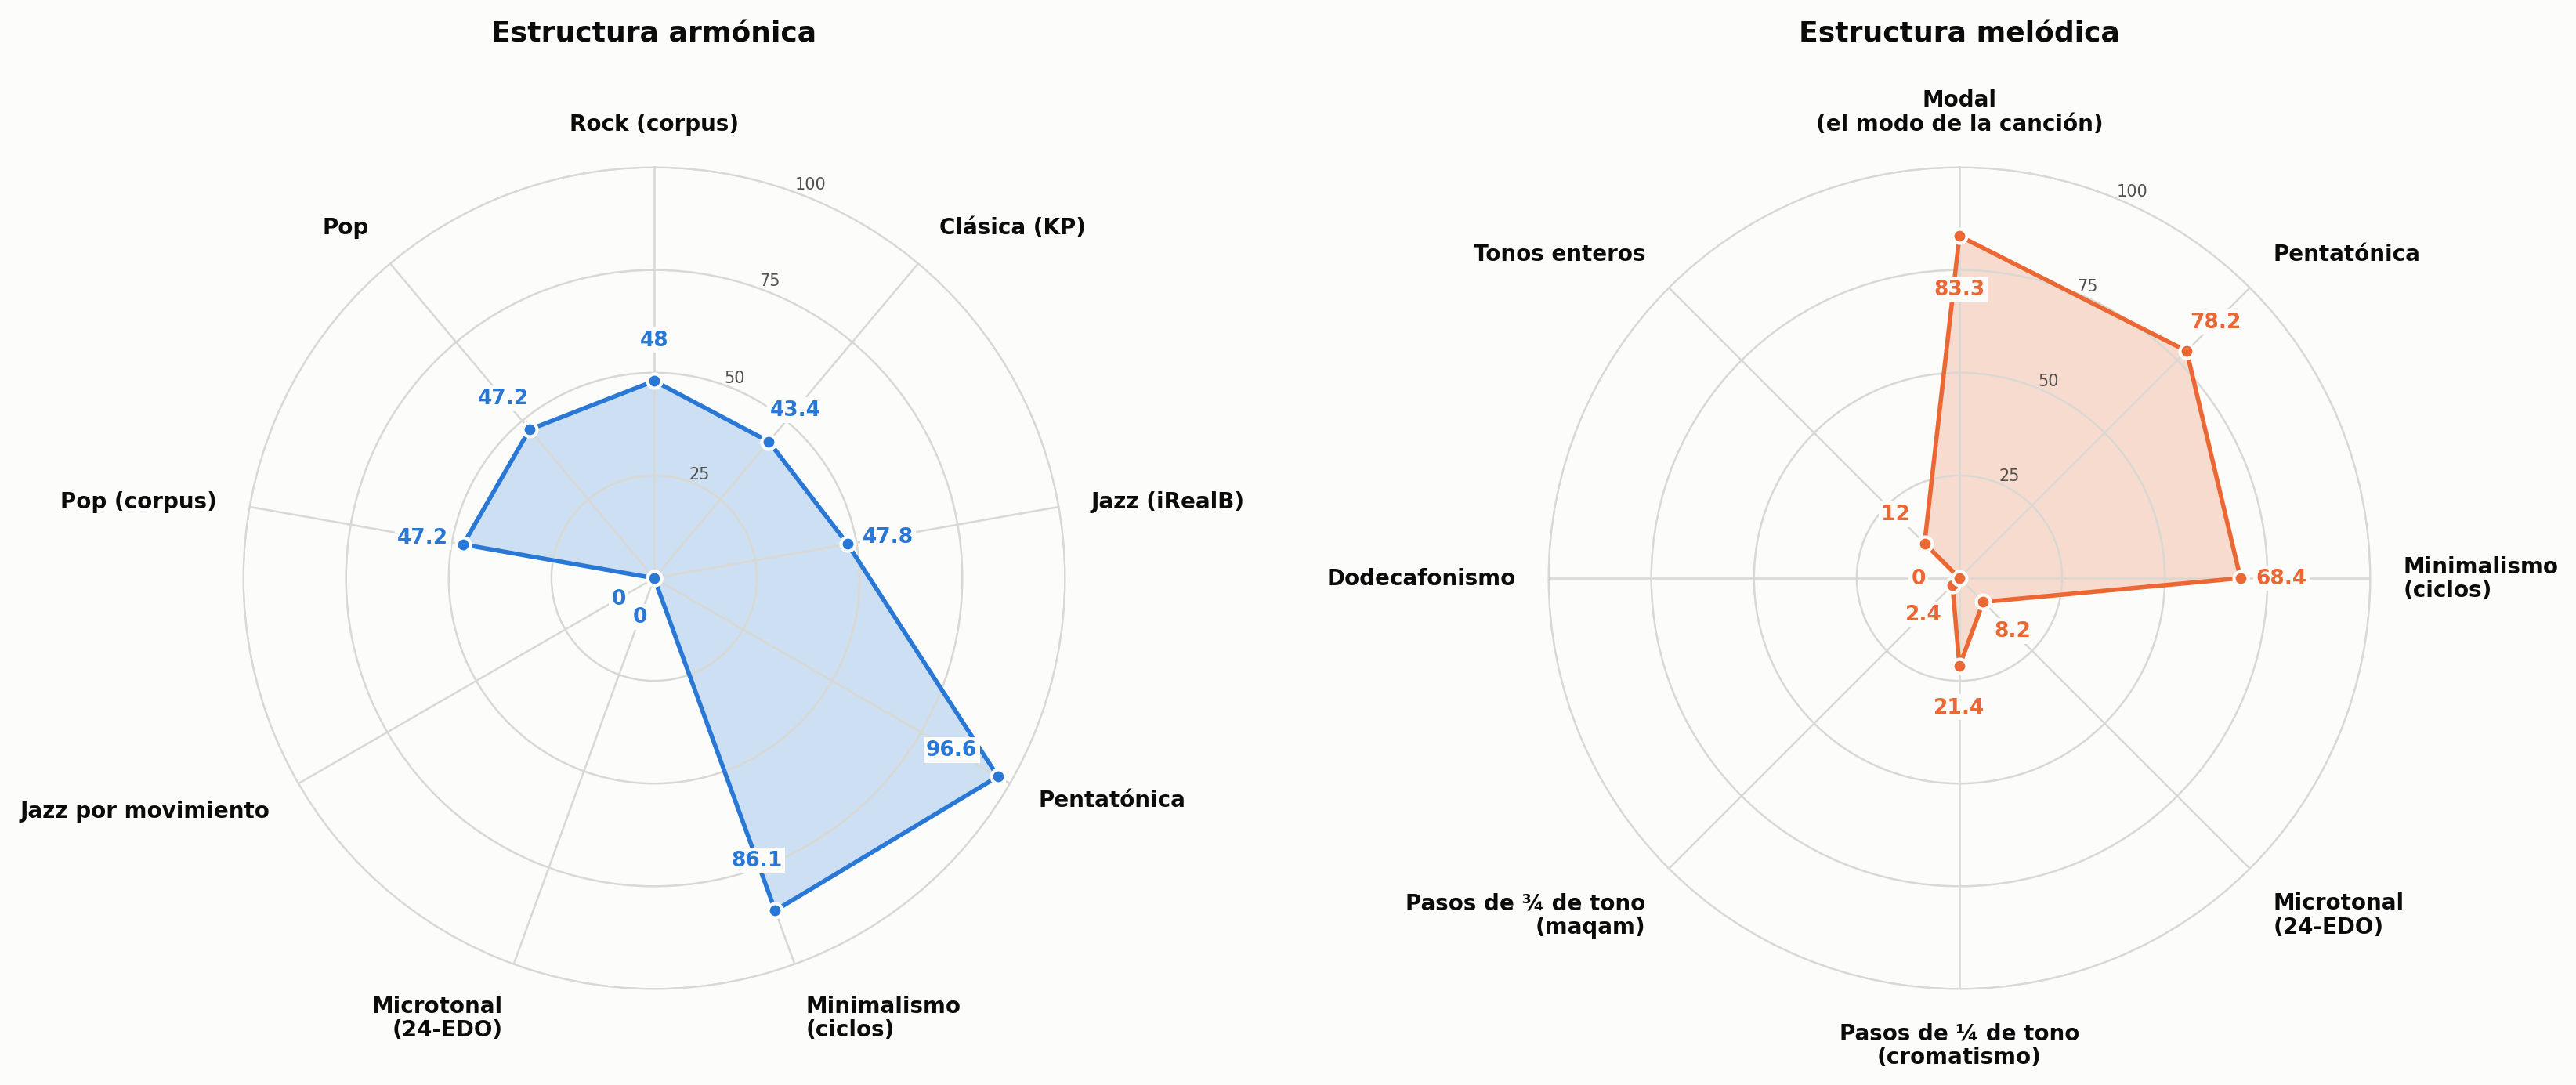
\includegraphics[width=\textwidth]{fabienk_radar_estilos.png}\\[0.5em]
  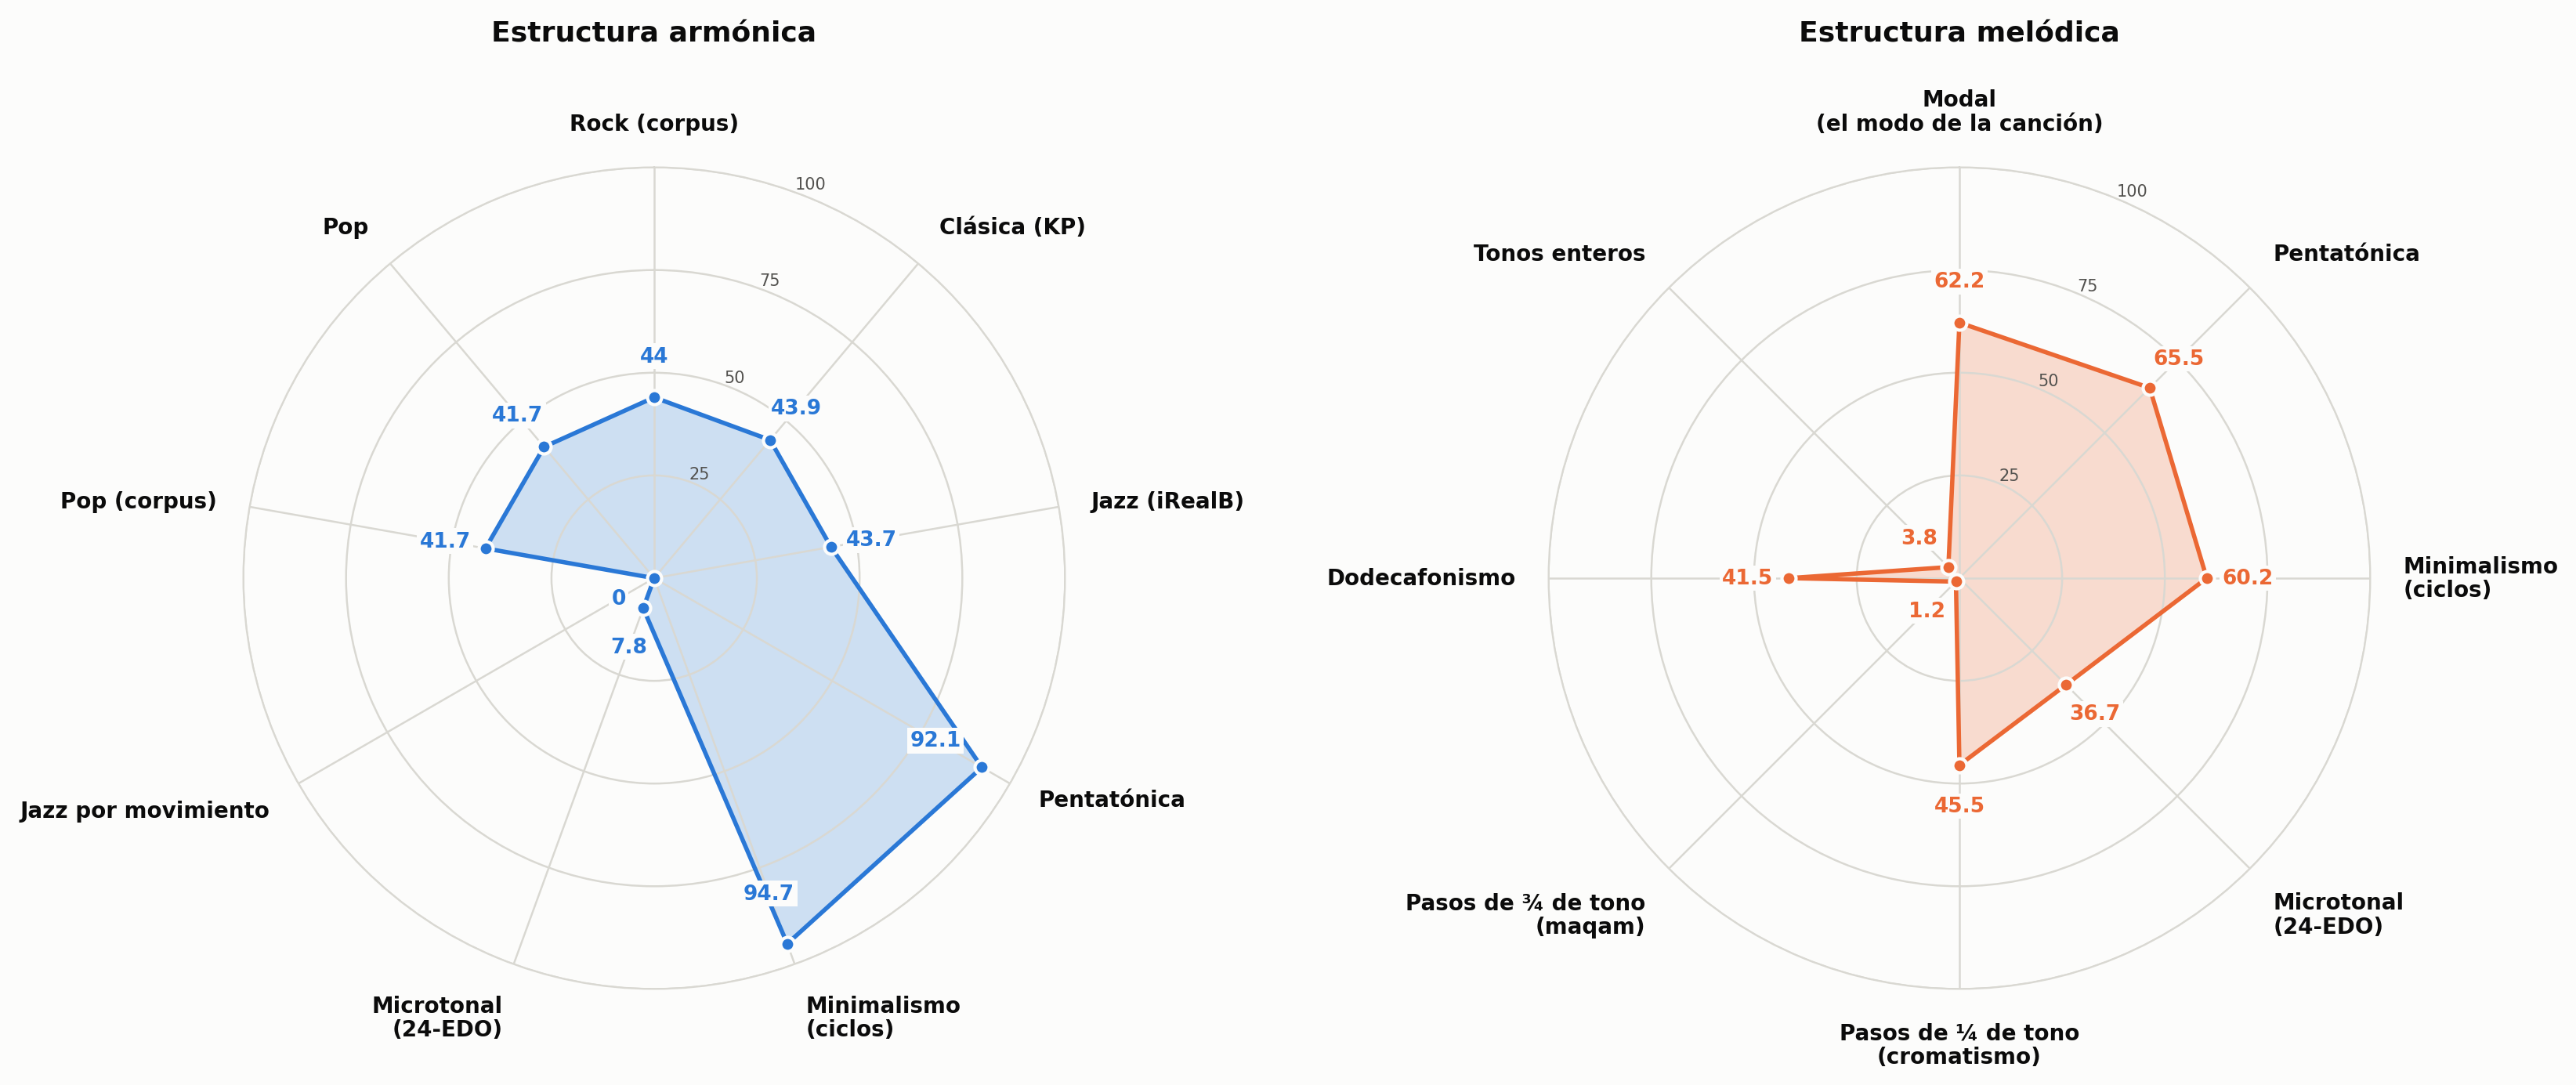
\includegraphics[width=\textwidth]{sarniezz_radar_estilos.png}
  \caption{Radares de estilo (versión descartada): Fabienk (arriba) y Sarniezz (abajo). Misma lectura que la figura~\ref{fig:radar-mata}.}\label{fig:radar-fab-sar}
\end{figure}

\begin{figure}[!htbp]
  \centering
  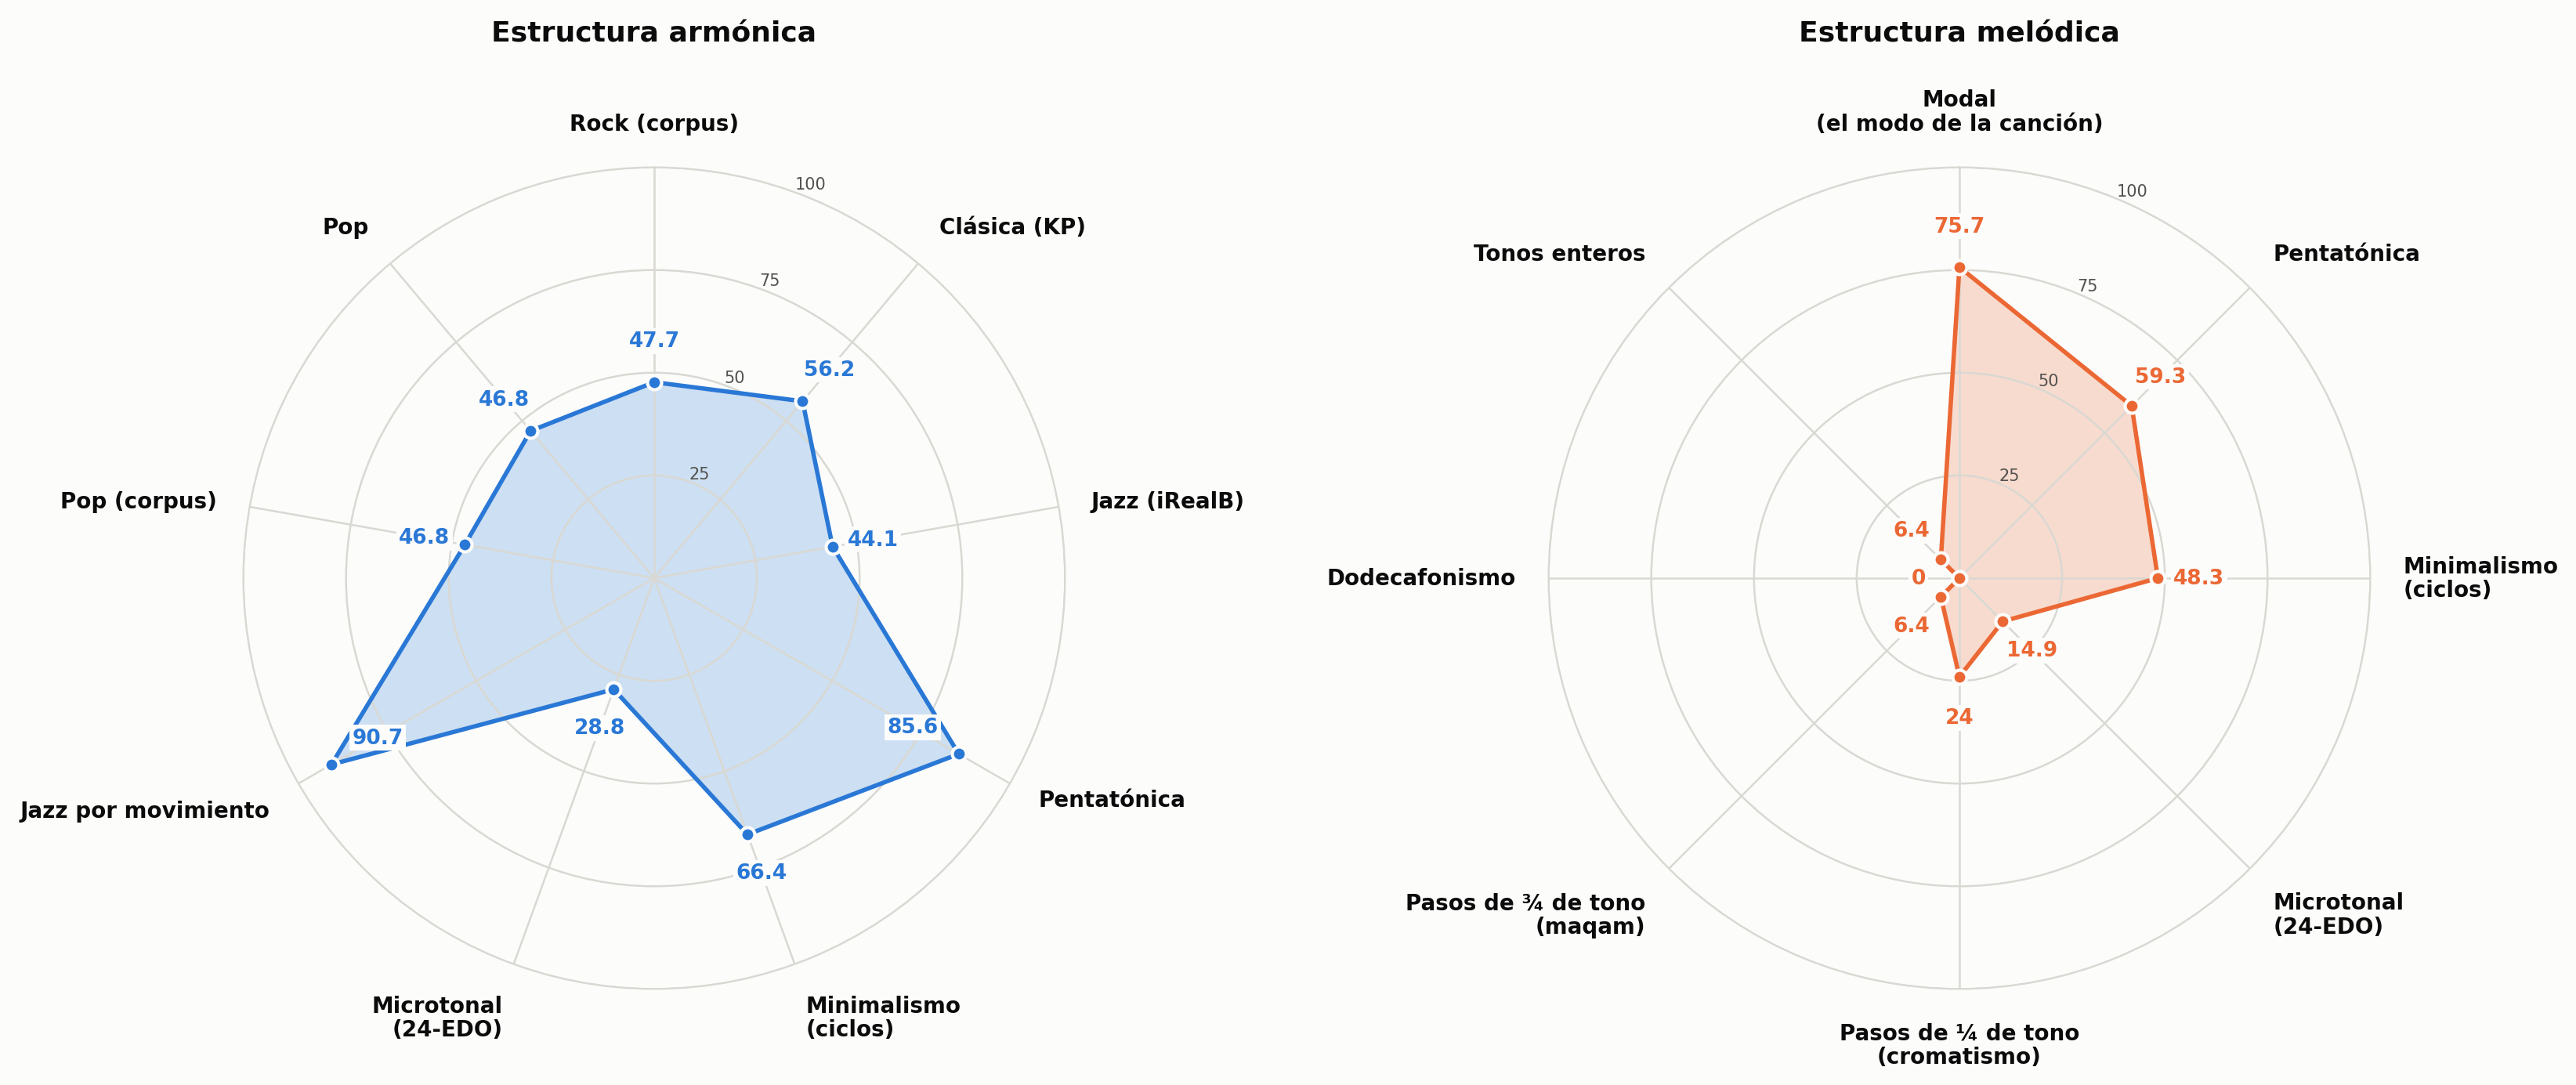
\includegraphics[width=\textwidth]{yor_zarad_radar_estilos.png}\\[0.5em]
  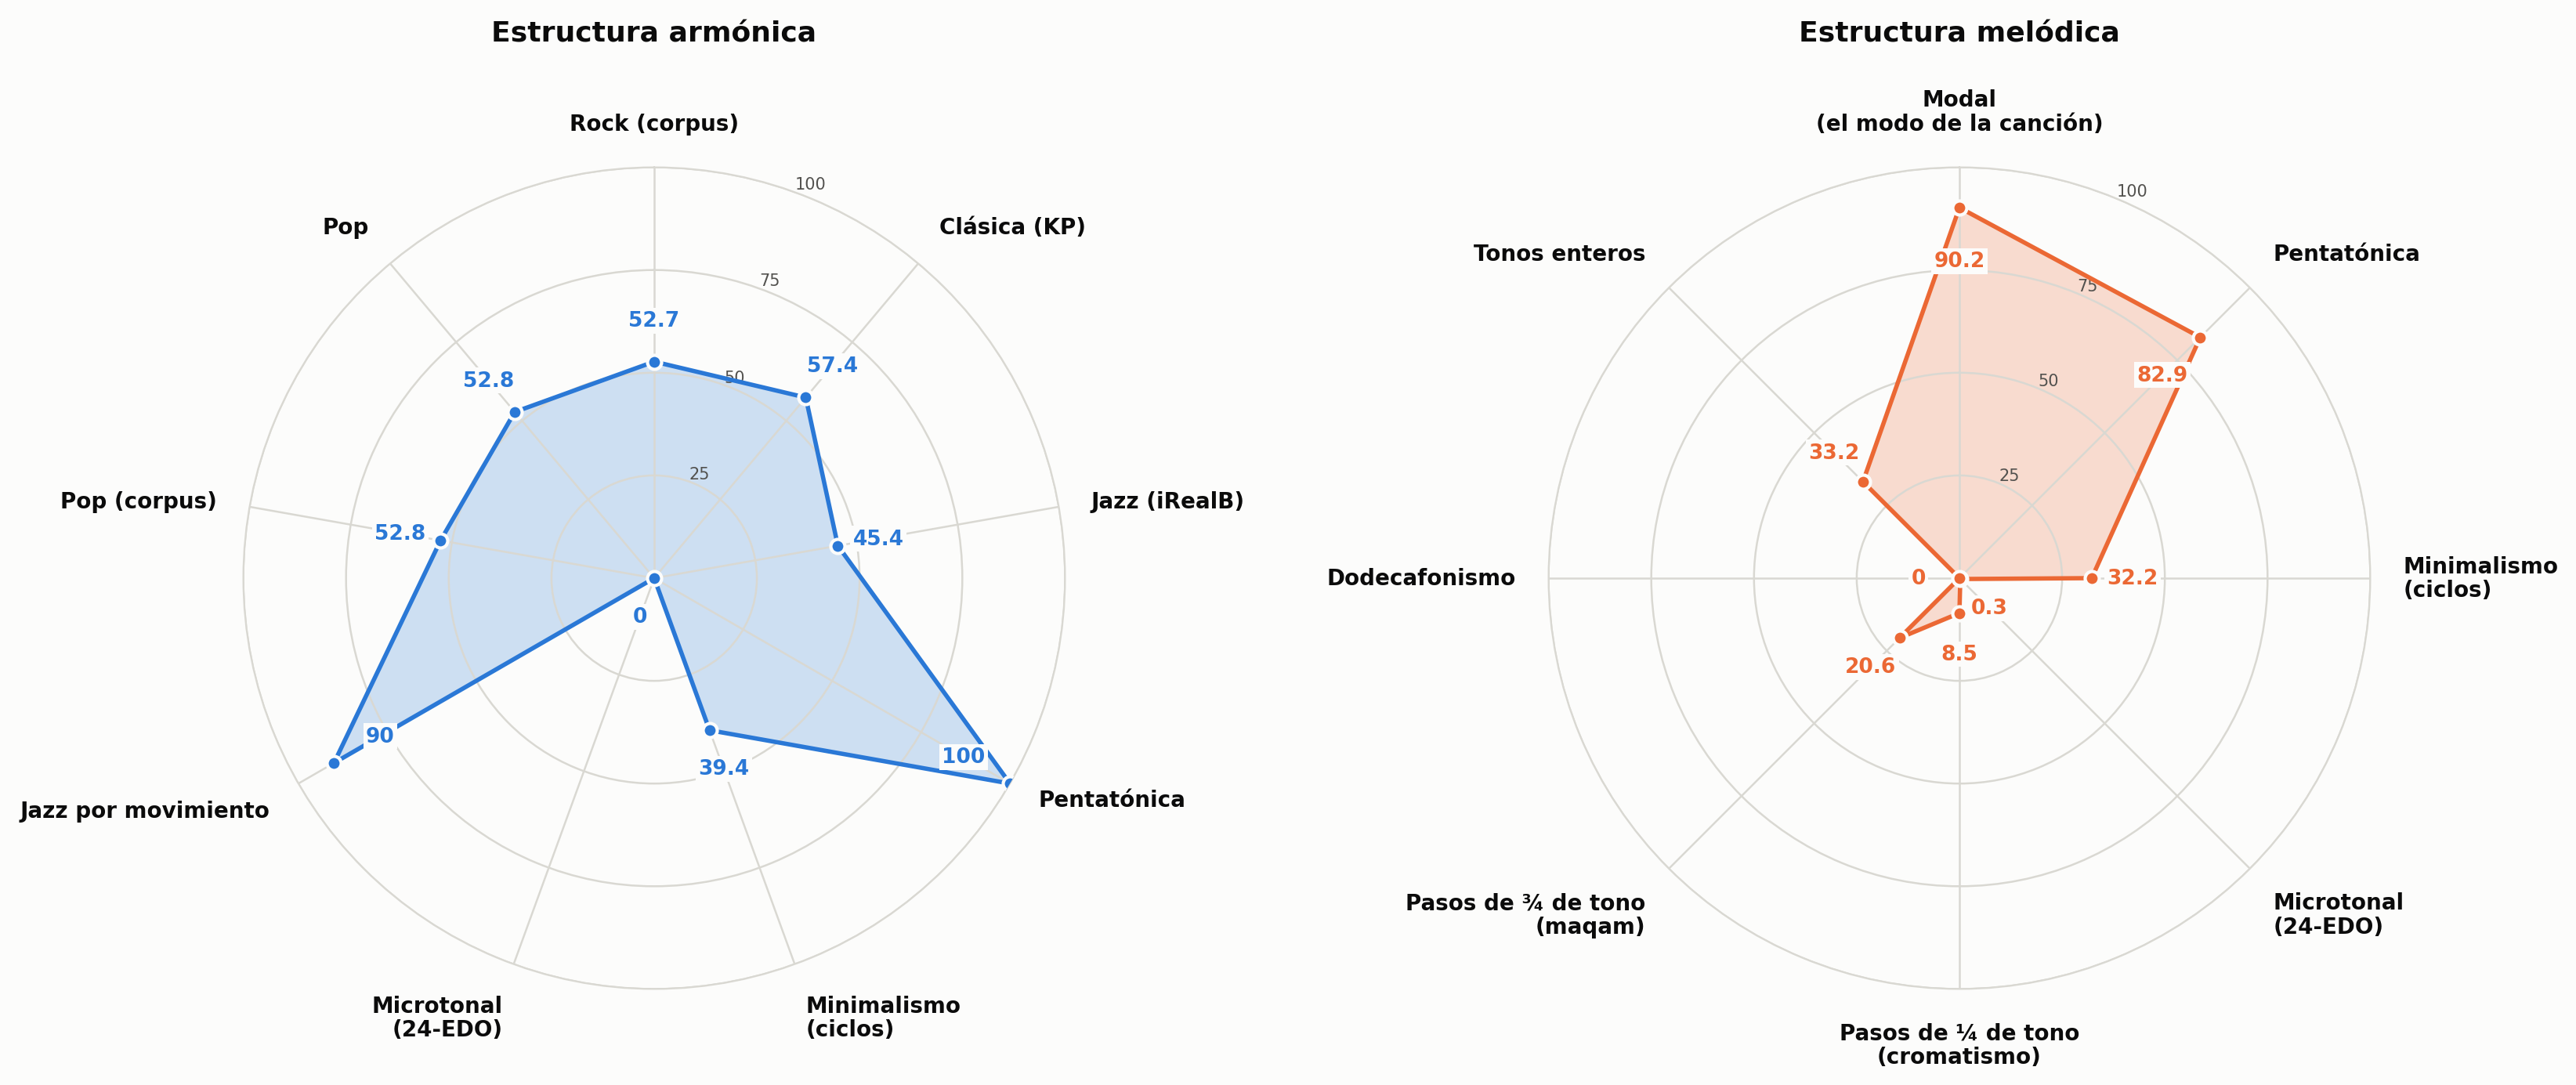
\includegraphics[width=\textwidth]{utzp_radar_estilos.png}
  \caption{Radares de estilo (versión descartada): Yor Zarad (arriba) y Utzp (abajo). Misma lectura que la figura~\ref{fig:radar-mata}.}\label{fig:radar-yor-utzp}
\end{figure}
